% REMEMBER: You must not plagiarise anything in your report. Be extremely careful.
\documentclass{l4proj}

    
%==============================================================================
% Put any additional packages here
% You can add any packages you want, as long as it does not alter
% the overall format (e.g. don't change the margins or the reference style).
%
\usepackage{pdfpages} % if you want to include a PDF for an ethics checklist, for example
\usepackage[normalem]{ulem}
%
%

\begin{document}

%==============================================================================
%% METADATA
\title{Mid-Air Gesture for Passenger Interaction in Cars} % change this to your title
\author{Catriona Murphy}
\date{February 16, 2021}

\maketitle

%==============================================================================
%% ABSTRACT
\begin{abstract}
    Cars are an ever-evolving technology, their makers constantly introducing new features to make the driver, and passenger, experience more pleasant. Mid-air gesture interaction is one addition that would allow backseat passengers to control these features with ease.  This has previously been studied in relation to drivers controlling aspects of a car but not backseat passengers. Often the passenger is still restricted as to what they can control and relies heavily on the driver. Incorporating mid-air gestures for use in the backseat of a car would allow the ever increasing range of luxury features to be utilised more fully without unnecessary distraction to the driver.
    
    In order to address this, different cars were investigated to discover which luxury features they incorporated within their cars. Gesture elicitation surveys were conducted in order to establish a set of gestures for these controls and these gestures were implemented using Python for a Leap Motion Sensor. An experiment was conducted so as to determine if the gestures were appropriate to be used for backseat passengers and where the best position for the sensor was. It was found that using mid-air gestures for backseat passengers has a lot of potential, but significant work will be necessary in improving many of the gestures so they are easier for all types of passengers to perform.
\end{abstract}

%==============================================================================
%% ACKNOWLEDGEMENTS
%\chapter*{Acknowledgements}
% Enter any acknowledgements here. This is optional; you may leave this blank if you wish,
% or remove the entire chapter
%
% We give thanks to the Gods of LaTeX, who in their eternal graciousness, 
% have granted that this document may compile without errors or overfull hboxes.
%

%==============================================================================

% EDUCATION REUSE CONSENT FORM
% If you consent to your project being shown to future students for educational purposes
% then insert your name and the date below to  sign the education use form that appears in the front of the document. 
% You must explicitly give consent if you wish to do so.
% If you sign, your project may be included in the Hall of Fame if it scores particularly highly.
%
% Please note that you are under no obligation to sign 
% this declaration, but doing so would help future students.
%
\def\consentname {Catriona Murphy} % your full name
\def\consentdate {19 February 2021} % the date you agree
%
\educationalconsent


%==============================================================================
\tableofcontents

%==============================================================================
%% Notes on formatting
%==============================================================================
% The first page, abstract and table of contents are numbered using Roman numerals and are not
% included in the page count. 
%
% From now on pages are numbered
% using Arabic numerals. Therefore, immediately after the first call to \chapter we need the call
% \pagenumbering{arabic} and this should be called once only in the document. 
%
%
% The first Chapter should then be on page 1. 

% PAGE LIMITS
% You are allowed 40 pages for a 40 credit project and 30 pages for a 
% 20 credit report. 
% This includes everything numbered in Arabic numerals (excluding front matter) up
% to but *excluding the appendices and bibliography*.
%
% FORMATTING
% You must not alter text size (it is currently 10pt) or alter margins or spacing.
% Do not alter the bibliography style. 
%
%==================================================================================================================================
%
% IMPORTANT
% The chapter headings and structure here are **suggestions**. You don't have to follow this model if
% it doesn't fit your project. Every project should have an introduction and conclusion,
% however.  If in doubt, your supervisor can give you specific guidance; their view takes precedence over
% the structure suggested here.
%
%==================================================================================================================================
\chapter{Introduction}

% reset page numbering. Don't remove this!
\pagenumbering{arabic} 

Cars are an ever-evolving technology, always incorporating new features to make the driver, and passenger, experience more pleasant. From being able to connect your phone via Bluetooth to listen to music, to built-in touchscreens to ensure interacting with navigation is both easier and less distracting, cars continue to evolve in new and interesting ways. There are also features that make the experience more relaxing. For example, heated massage chairs and heated steering wheels enhance comfort for the driver, particularly in cold conditions.

Considering the touchscreen, it is primarily there for the driver. Passengers in the rear of the car have very little control over the choice of music, the volume at which it is played or the temperature in the car. They instead must rely on the driver to perform actions to make such adjustments, actions which could be distracting and potentially dangerous should they take their eyes off the road. 

Many high-end cars such as the \cite{Bentley_2021} Flying Spur include numerous features for backseat passengers including a remote control to interact with the centre console and a rear infotainment system. Although this is a step forward in giving backseat passenger more freedom and a higher level of luxury, many systems continue to rely on touchscreens, buttons or handles.

One way of overcoming this inconvenience is to use mid-air gestures. While their use in cars is not commonplace, they have previously been researched and trialled to demonstrate how they could ease the driver's experience and thus enhance the safety of their driving. This study, however, will not focus on safety but only on the quality of the passenger's experience. We will investigate which cars have luxury features and then find out what sort of gestures passengers would perform to execute these. Additionally, we will investigate the suitability of performing these gestures in the backseat of a car.

\section{Motivation}
Mid-Air Gestures are a growing technology that have only recently been integrated in cars, BMW being the first brand to incorporate mid-air gestures for their drivers (\cite{Dow_2017}). There are 8 different gestures within the BMW gesture set, and, by gesturing close to the centre console, drivers can answer phone calls, adjust volume and perform many more tasks (\cite{Rommel_2020}). There are several other car models that have incorporated gesturing including Jaguar, Mercedes-Benz, and Volkswagen (\cite{Dow_2017}). However, their gesture sets are more limited than the BMW.

In all of these cases, the gestures were only available for the driver to perform. Added features, which make the passenger's experience more relaxing and enjoyable, are a necessity for luxury cars. This is especially important if a car is chauffeur driven or self driven (if such cars become mainstream and widely trusted). 

However, using mid-air gestures does not only need to be seen as a luxury technology but a family friendly one. According to the \cite{Department_for_Transport_2017}, 3\% of all car accidents are caused by a driver being distracted by someone else in the vehicle. If the backseat passengers were able to have full control over what they wanted to do then how often they distract the driver could be reduced and therefore lead to safer driving.

\section{Aims}
Having established the motivations, a survey was conducted to ascertain which gestures would be most appropriate for use in the backseat of a car. These gestures were then trialled using a Leap Motion gesture sensor. Using this set of gestures, an experiment was conducted to answer the question: how suitable are these gestures for performing in the backseat of a car?
To explore more deeply, this question will be split into multiple parts: 
\begin{itemize}
\item Which gestures do backseat passengers associate with actions they can do in the backseat of a car?
\item Which gestures can be implemented using the Leap Motion sensor?
\item How well are the gestures performed while sitting in the backseat of a car?
\end{itemize}

\section{Structure}
This chapter discusses the motivation and aim behind “Mid-Air Gestures Interaction for Passengers in Cars” and, in doing so, clearly outlines the objectives of the project and why the use of mid-air gestures could be beneficial for backseat passengers. The rest of the paper is structured as follows:
\begin{itemize}
\item Chapter 2: Background Research. This chapter discusses the different cars that could be used and research on mid-air gestures, both in cars and not.
\item Chapter 3: Requirements Analysis. This chapter discusses the tasks undertaken to gather the requirements for this project.
\item Chapter 4: Design Process. This chapter outlines the process behind designing the experiment
\item Chapter 5: Implementation. This chapter explains how different aspects of the experiment were implemented
\item Chapter 6: Experiment and Evaluation. This chapter documents the experimental process and results.
\item Chapter 7: Conclusions and Future Work. This chapter summarises the work done and discusses the potential future work for the project.
\end{itemize}



%==================================================================================================================================
\chapter{Background}

\section{Luxury Cars}
\label{section:luxuryCars}
Nowadays, there are many different technologies that can be incorporated into cars from more basic climate control to infotainment systems that can play music, videos and connect to smartphones (\cite{Svangren_Skov_Kjeldskov_2017}). This is a major component in modern car manufacturers' attempts to attract new customers to their products. \cite{Christou_2019} cites research which concludes that the more technologies that are incorporated into a car, the more attractive it is deemed - 55\% of car purchases are influenced by the technology that a car has.

Some cars that have these “luxury” features include Rolls-Royce, Bentley, Mercedes, and Range Rover. However, there are many more that could be considered.

The features which can be offered in two of the Rolls-Royce range, the Dawn Black Badge and Ghost, include heated seats, lumbar support, and climate control. DVD and CD players which can be controlled with a remote control and Bluetooth connectivity can also be included (\cite{CarDekho_2020}). The Rolls-Royce range lacks a rear entertainment system which would be needed to incorporate a mid-air gesture system as the passengers would require visual feedback so that they know they are performing the gestures correctly.

The Bentley Flying Spur model also includes heated seats, lumbar support, and climate control. However, its climate control is 4 zone which means that each seat in the car can be a different temperature to suit the individual comfort needs of all passengers.  Furthermore, it also has a rear entertainment system which, as previously mentioned, is required for the inclusion of mid-air gestures. The Flying Spur connects to smartphones and has built in GPS (\cite{Bentley_2021}).

\begin{figure}[!htb]
    \centering
    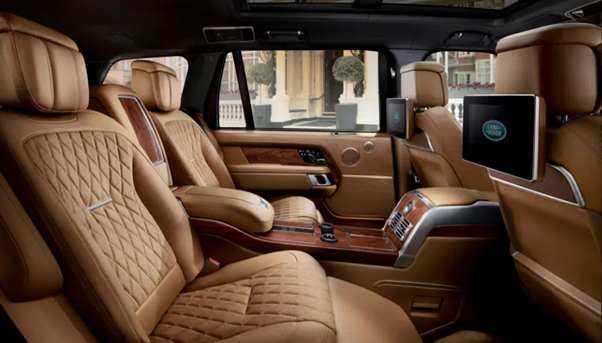
\includegraphics[scale = 0.5]{images/rangeRoverInterior.png}
    \caption{Backseat Entertainment in Range Rover Autobiography (\cite{Finnerty_2017})}
    \label{fig:rangeRoverInterior}
\end{figure}

The Mercedes S-Class is similar to the previous cars in terms of features. However, it also has ambient lighting, massage chairs and four-way lumbar support (\cite{Mercedes}). Range Rover has similar features (\cite{Range_Rover}). Obviously, feedback does not only have to come in the form of visual aids but the passenger would be facing that direction so they would be able to see it easily. The Range Rover rear entertainment systems, as shown in Figure \ref{fig:rangeRoverInterior}, have large screens and are placed at passenger's eye level on the seat. This also shows the champagne cooler that the Range Rover Autobiography includes, situated in between the two back seats.

It was decided that the Range Rover would be the best option for the project to be based on. Although still a high-end luxury brand, it is more accessible to the average consumer with the total sales in 2019 of Bentley’s and Rolls-Royce being 11,006 (\cite{bentley_Bekker_2020}), and 5,152 (\cite{Rolls_Bekker_2020}) respectively, in comparison to a total of 396,105 cars sold by Land Rover in 2019 (\cite{Statista_2020}). Furthermore, while the Land Rover's features were the basis of the gestures used in the experiment, this does not mean they are limited only to being used in a Land Rover. These features, as described, have been used in numerous car brands and this will continue to be the case.


\section{Gesture Elicitation}
According to \cite{Villarreal_Narvaez_Vanderdonckt_Vatavu_Wobbrock_2020}, a gesture elicitation survey is a useful tool in learning about how users will interact with different devices and applications. \cite{Vogiatzidakis_Koutsabasis_2018} claim that the “main goal of an elicitation study is to elicit appropriate gestures for mid-air interactions”. These gestures could then be used to build a system or simply to understand how a user may think.

Many studies on gesture elicitation have been done including studies on surface gestures (\cite{Morris_Wobbrock_Wilson_2010}), TV (\cite{Vatavu_Zaiti_2014}) and wall displays (\cite{Wittorf_Jakobsen_2016}). 

The gesture elicitation survey for the TV was especially interesting as a Leap Motion sensor was used. The experiment required participants to sit 2m away from a TV and they were presented with 21 referents in random order. The referents are the effects of a gesture command. Each participant was given a trial run during which they were able to propose a gesture for each referent. They were then asked to go through it again and perform their gesture so it could be recorded and analysed. After the experiment, the participants were given the referents again and asked to recall their own gesture. They were then asked to rate - on a scale of 1 to 5 - how well it fit the referent. They were also asked to perform their own gesture again so that the evaluator could rate how well they remembered it (\cite{Vatavu_Zaiti_2014}). This method of gesture elicitation was very thorough as they asked the participants to rate their own gestures as well as create them. This gives a deeper understanding of how well a gesture may work. This elicitation survey resulted in 378 gestures which could then be analysed to create a condensed data set that could be used with a TV.

\begin{figure}[!htb]
    \centering
    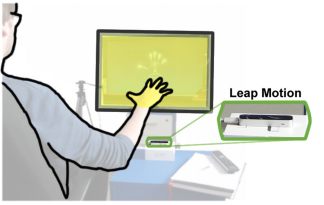
\includegraphics[scale = 0.5]{images/leapTV.png}
    \caption{Leap TV Gesture Elicitation Set Up (\cite{Vatavu_Zaiti_2014})}
    \label{fig:leapTV}
\end{figure}

Figure \ref{fig:leapTV} shows how the Leap TV gesture elicitation was set up. Although the TV screen is considerably larger than a tablet screen in a car, the set-up could be similar to how performing gestures in cars would work. The participant performs the gestures facing the screen and receives immediate feedback from the screen. This is a very important feature to consider as a user will want to know if they are doing something wrong in order to fix it. The user will also want to receive confirmation that they are performing the gesture correctly so they can stop.

One study by \cite{May_Gable_Walker_2017} discusses eliciting gestures for drivers using mid-air gestures. It includes 2 different studies: an elicitation survey and a workload survey. The participants were sat in a driving simulator,  presented with tasks and were asked to propose a hand gesture or sign that related to the output on the screen. This is known as a ‘theatre approach’. Having visual and auditory feedback, prompts the participant to perform gestures that are more directed towards the outcome rather than more abstract gestures. It is important to note that all 14 participants had a driving licence as the gestures would be used by drivers if they were incorporated into real cars. Once this study was completed, the gestures were categorised into groups of similar gestures, and the top four gestures for each task were identified for the workload survey which asked participants to rate different aspects of the gestures for each task.

The study on eliciting gestures for wall interfaces could be more relevant towards backseat passengers performing gestures as they have a wider range of motion than drivers  and the sensor could be in front of them, on the back of the chair. \cite{Wittorf_Jakobsen_2016} performed a think-aloud gesture elicitation study where the participants were shown a sequence of images (the referent) to then produce a gesture which they thought related to it. However, unlike other gesture elicitation surveys, the participants were asked to perform as many gestures as they could think of that related to the referent. Once they had exhausted all their gestures, they were asked to pick their favourite. This was followed up with an interview. 

\begin{figure}[!htb]
    \centering
    \begin{subfigure}[b]{0.45\textwidth}
        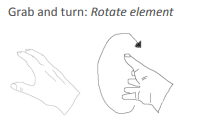
\includegraphics{images/rotateElement.png}
        \caption{Rotate an Element}
        \label{fig:rotateElement}
    \end{subfigure}
    \begin{subfigure}[b]{0.45\textwidth}
        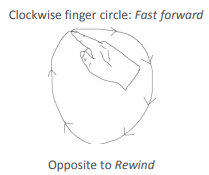
\includegraphics{images/clockwiseCircle.png}
        \caption{Clockwise Circle}
        \label{fig:clockwiseCircle}
    \end{subfigure}
    \caption{Illustration of Physical Manipulation Gestures (\cite{Jakobsen_2016})}
    \label{fig:gestureSet}
\end{figure}

These gestures were categorised, and the most common type of gesture performed was in the physical category. This meant that the participant acted as though they were physically handling an object as shown in Figure \ref{fig:gestureSet}. 

This could potentially affect how users interact within a car, as the majority of what they would interact with would have strong physical actions to accompany them, for example, rolling down the window or adjusting the volume. Consequently, this could lead to users having to perform gestures that are similar in terms of the effort required to perform the actual task.

\section{Mid-Air Gestures}

A good use of mid-air gestures is for household appliances such as thermostats. The challenge with this sort of device is that they don’t tend to ever give immediate feedback as a house needs to either warm up or cool down (\cite{Freeman_Brewster_Lantz_2015}). In this research, two different gesture inputs were compared in which it was found that using a dial motion was more precise than using a punching motion. It was also discovered that users found gesturing a lot more convenient than more conventional methods of interaction. This aligns with the motivation behind this project in that using mid-air gestures in cars would not be considered a necessity but could be significantly more convenient for users. Additionally, this research provides ideas on how users could interact with air conditioning in cars as it is a similar concept. 

A similar idea to this is Google’s Nest which is a thermostat which will automatically light up when someone is near. While it does not actually use mid-air gesturing to make adjustments, it does use a person’s movement to turn on (\cite{Haselton_2020}).This is helpful in understanding that mid-air gestures do not need to be used to perform complicated tasks but could be used to make a straightforward task easier.

One study researched how users could interact with seven different household items using mid-air gestures. \cite{Vogiatzidakis_Koutsabasis_2020} chose TV, lights, and blinds along with other appliances to discover how well people could interact. In this study, users were provided with training so they could learn how to perform the gestures and a Kinect was used to recognise these gestures. Since there were so many devices being worked with, the user had to perform a “registration” gesture to activate the device they wished to interact with. This is an interesting way to interact with different objects in a room. Rather than trying to invent several unique gestures, the only gestures that needed to be unique are the ones to activate the interaction with a certain object. Following this, the other gestures could be reused. 

Within the majority of literature reviewed, age was not taken into account when the studies were being conducted. The most important feature to researchers was to ensure that there were enough participants in each study with little focus given to their age. However, \cite{Cabreira_Hwang_2016} noticed this gap in the literature and investigated how well older people perform mid-air gestures. This is especially important when considering the use of mid-air gestures in cars as car passengers can be any age. Furthermore, interest in latest technology in cars is not limited to a particular age group. This shows that, when researching a new technology which contains potential safety hazards, considering all age groups and categories is very important and worthwhile. It can make mid-air gestures more universally available and appropriate for any user. The findings from this research suggests, however, that there is very little difference in the way that older novice users perform mid-air gestures and that they are just as competent as younger users. The only issue observed was that they lack the confidence while performing them which could potentially deter them from using them while in a car as they lose hope in the gesture working. 

\begin{figure}[!htb]
    \centering
    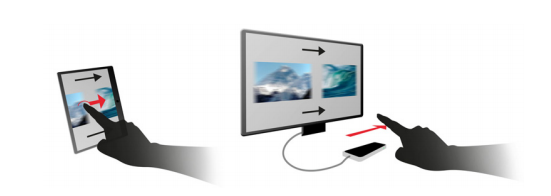
\includegraphics[scale = 0.6]{images/gameGestures.png}
    \caption{How the children were asked to interact with the game. (\cite{Moser_Tscheligi_2015})}
    \label{fig:gameGestures}
\end{figure}


\cite{Moser_Tscheligi_2015} studied how well children interacted with an online game while performing mid-air gestures. It involved 20 children aged between 11 and 14 and they used a Leap Motion sensor to track their finger movements.The experiment compared the use of traditional touch based input and mid-air gestures and, as shown in figure \ref{fig:gameGestures}, the participants were instructed to swipe their finger across the screen either by touching it or hovering over the sensor in front of them. The results were positive, showing that three quarters of the participants were keen to play the game again using mid-air gestures. However, controlling the game using mid-air gestures was found to be more difficult than touch but was just as engaging. Mid-air gestures made the overall game experience more "fun" and "great" than using touch. This is encouraging as it shows that younger people can interact with interfaces that use mid-air gestures and that they enjoy them. It was found however, that with using the Leap Motion, children found it difficult to input precise gestures and that they also tended to move their hands away from the sensor and towards the screen which meant the Leap Motion could not recognise their finger. These issues show that incorporating mid-air gestures into children's everyday lives is not a perfect solution but it does certainly have potential.

\cite{Hessam_Zancanaro_Kavakli_Billinghurst_2017} present research on identifying which mid-air gestures are the safest and most accurately performed whilst driving. They do not focus on how the feedback makes driving safer while gesturing but instead focus on how the type of gesture affects performance and therefore affects the overall safety inside the car. To do this, they performed an evaluation study to assess the appropriateness of their gesture set by asking participants to rate the usability of a gesture while driving. An acceptance index was created and from this the gestures could be considered “acceptable”, “confusing” or “inappropriate”. The results showed that, even if a mid-air gesture is deemed acceptable while driving, that it may still not be safe to do so. For instance, a mid-air gesture to turn off the car could end up causing a catastrophic accident if the driver accidentally performed it while driving on a motorway and the car stops. Furthermore, it is shown that, even if a gesture helps perform a task, it still is not appropriate to be performed while driving as it could be confusing.  This type of research could potentially inspire a wide range of future research due to it creating a set of gestures “optimised” for driving.

\cite{Freeman_Brewster_Lantz_2016} presented a study on how users “address” a system while interacting with it and discuss how most users automatically know how to interact with a touchscreen device or buttons, but with mid-air gesture systems it is not as clear, especially if there is more than one in the room. Addressing a system involves the location of where a user should gesture and how they should direct their input in a non-disruptive way. The experiment involve mobile devices and a wall dial. Freeman explains that, when using mid-air gestures, the input space becomes much larger than the device and users are not as restricted. When using them in cars, users will still be restricted by the dimensions of the car but would still have a greater input field than before. 

It is important to acknowledge which gestures are most commonly used currently. \cite{Cabreira_Hwang_2015} compared different applications that were specifically created for mid-air gesture interaction use and the gesture set within these applications. This comparison was done for Microsoft Kinect, Leap Motion and Myo Armband applications. However, only free applications could be considered which did restrict the amount of apps that could be looked at. The gestures found were categorised in three ways: navigation, selection and triggering an action. Fifteen common gestures were identified and the overall most common type of gesture involved pointing followed by waving and swiping. These gestures are fairly basic so it is understandable that all three gesture sensors recognised them. Myo Armband was found to be the most limited while the Leap Motion has a wider range of options. This shows that it would be a good sensor to use if it was necessary to perform gestures for a large amount of actions or, if necessary, for there to be no duplicate gestures in a fairly small set. 

\subsection{Feedback from Mid-Air Gesture Interaction}
\cite{Shakeri_Williamson_Brewster_2017} presented a study on new ways to present feedback in cars while the driver is performing mid-air gestures. This paper focused on moving away from visual feedback and towards alternative channels that are less important to driving and therefore would result in less distraction. These included audio, tactile, and peripheral vision. 

Tactile feedback in the form of haptics is further explored by \cite{Shakeri_Brewster_Williamson_Ng_2016} where the use of solenoid pins is studied for its appropriateness and ease of use. This has been named cutaneous push and it focuses on the three most sensitive areas on a palm which would be touching a steering wheel while driving (Figure \ref{fig:cutaneousPush}).  This is a new concept that has not been explored before as haptics tend to come in the form of vibrations which can confuse drivers and cause more problems than visual feedback would. Overall, it was found that this new way of providing feedback was safer and resulted in less “eyes-off-the-road time” which is very important for drivers as the longer they are looking away from the road, the more likely they are to cause an accident.

\begin{figure}[!htb]
    \centering
    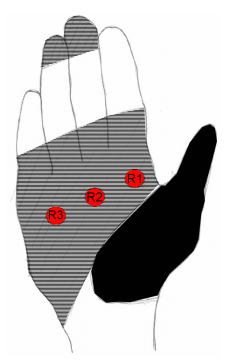
\includegraphics[scale = 0.5]{images/cutaneousPush.png}
    \caption{Three most sensitive areas on palm of right hand. (\cite{Shakeri_Brewster_Williamson_Ng_2016})}
    \label{fig:cutaneousPush}

\end{figure}

\cite{Shakeri_Williamson_Brewster_2018} further explore new feedback types in the form of ultrasound haptics. Again, this appears to be an area that is not well researched regarding feedback in cars. However, it has been analysed to further understand how well people can sense ultrasound haptic shapes and buttons. This, alongside other feedback methods researched, indicate that technology is constantly evolving to make our experiences while driving safer and more convenient.

In a study by \cite{Freeman_Brewster_Lantz_2015}, “Do That, There”, a new technique was discussed where “There” indicated where the users should perform their gestures and “Do That” indicated showing the users how to direct their input and ensure that all gestures are intentional. The study aimed to find a solution to provide meaningful feedback on different types of devices when mid-air gestures are used to interact. The use of ‘smart’ thermostats in households were examined: with little to no screen space to provide feedback, alternative methods of feedback were investigated to determine whether they help users address and interact with the devices. There were three experiments with the first exploring the “There” section of the technique. This is done to direct the participant to gesture in the right place. Participants were given 15 tasks to do with their finger being tracked over a mobile phone. These tasks were done 7 times, each with a different feedback method. It was found that auditory feedback resulted in participants placing their hands in the right position more successfully. Visual feedback, however, was shown to increase how long it took for a participant to complete a task.\\ The second experiment required users to perform different gestures to match the light display on a smart thermostat. This was categorised as the “Do That” part of the experiment. The participants found that auditory feedback was the most effective but that tactile feedback was still helpful, especially if audio could be inappropriate at certain times.\\
Finally, the last experiment combined the previous two so that the “Do That, There” technique could be investigated fully. The thermostat was used again but this time, the participants had to work out where they were to perform the gestures and match the gesture. If they did match, then they had to hold it for as long as possible. It was discovered that users performed best when all feedback methods were given to them simultaneously and that they found this less difficult. \\
This research shows that using different feedback methods simultaneously can aid users in performing the correct gestures and knowing where to perform the gestures. However, it is also clear that providing the most appropriate form of feedback is very important, especially if it is impossible to provide multiple types at once. 

\section{Conclusion}
As mentioned previously, there are many luxurious cars which feature many different technologies which could be controlled using mid-air gestures. Range Rover and the Mercedes S-Class were found to have the widest variety of features so were the best options to choose from when deciding which vehicle the project should be based on. 

Following this, it was important to investigate different gesture elicitation surveys and discover what other researchers had discovered about gesture elicitation in order to find the best way to perform them. Unfortunately, due to Covid-19, the methods used above would mostly be unsuitable as they were all done in-person. However, the general ideas behind them were useful as most of them consisted of the users having to rate the gestures they performed to obtain an idea behind what they were thinking and if they did find them appropriate for each scenario. A gesture elicitation survey is essential in discovering how users interact with different systems and it is important to receive their input before creating a system as it may not be intuitive for users. 

Mid-air gestures are becoming a more popular way to interact with systems in the household and while driving. These sort of interactions have been shown to be fairly basic with interactions including adjusting temperature and controlling the TV. It was also found that the effectiveness of performing mid-air gestures was not limited to a certain age group and that people of all ages can use them effectively. This is important to acknowledge as people of all ages can be backseat passengers and, as children are regularly backseat passengers, mid-air gestures need to be manageable for them. One study found that children enjoyed performing the gestures but had difficulty being precise with their gestures. They still managed to play the game in the study which shows they were determined to continue using them. Older users were found to be hesitant while performing mid-air gestures but were just as competent as younger, more experienced users. It is important to know that a system can be used by people of all ages so that it can reach a wide audience that will want to engage with it. 

Safety is a big concern when it comes to drivers performing mid-air gestures as they have the potential to direct focus away from the road. This is not such a big a concern for backseat passengers. Most important for them is that they know how to interact with a system and that it is easy for them to understand where they need to gesture and what gestures will trigger an action. A useful way to aid passenger's understanding is to provide them with feedback. There are many new forms of feedback that are evolving. Haptics such as ultrasound or cutaneous push have been proven to make the drivers experience, while performing mid-air gestures, safer. However, feedback such as audio and visual have been shown to be just as effective and may be more suitable for backseat passengers as there is less concern about distraction.

The literature presented does not include any research on mid-air gesture interaction for passengers in cars and this is a clear gap in the field. Using this research will aid the investigation on how users could interact with a system that uses mid-air gestures in the backseat of a car. Knowing what common gestures are currently being used in other fields, and the fact that people of all ages are able to effectively use systems with mid-air gestures, offers promise that the research will produce positive results.

%==================================================================================================================================
\chapter{Analysis/Requirements}

\section{Gesture Elicitation}
In order to gain an insight into what mid-air gestures people thought would be most appropriate for the controls outlined in Section \ref{section:luxuryCars}, a gesture elicitation survey was undertaken. The aim of this experiment was to learn about what gestures people associated with different controls in the backseat of a car when there is a sensor placed either in front of them, on the centre console or on the door besides them. 

Prior to participating in the experiment, all participants signed a consent form and read an information sheet (Appendices \ref{section:ConsentGE} \& \ref{section:inforSheetGE}) so that they knew exactly what they were participating in. Before the survey started, the participants were also read an introduction script which further explained what they had to do (Appendix \ref{section:introScriptGE})

The experiment required each participant to sit in the backseat of their car, if they had access to it. However, if a participant was unable to use their car for whatever reason, sitting on any chair in their house was appropriate. Ultimately, all participants sat in their house as they were all using their computer, or it was dark outside. This could potentially make the data received not as reliable as had been originally hoped due to there being inconsistencies with the environment. Realistically, different cars have multiple types of seats so, unless the survey could have been done in-person, no-one’s conditions would have been similar. Furthermore, everyone was restricted to a desk chair and the exact position of the sensor was explained so they knew where their hands should be positioned.

There were 20 participants involved: 9 females and 11 males. The gesture elicitation survey was completed over Zoom and each participant was recorded so their elicited gestures could be analysed later. Participants were asked 10 questions (Appendix \ref{section:GESurveyQ}), some of which had multiple parts. This led to a total of 22 questions. It was decided that the questions would be done in a set order, ensuring consistency amongst participants, while randomising where the sensor was positioned. 

However, order-effect bias could have occurred due to the questions being kept in a set order. Order-effect bias is when the placement of a question in a survey would influence the way the participant reacts to it (\cite{Perreault_1975}). In this scenario, participants may want to use the same gesture more than once but decided against it because they may think they need to perform unique gestures.

The participants were made aware that they were being recorded and they could stop participating and have their data removed if they wished and at the end of the survey they were read a debriefing script (Appendix \ref{section:debriefScriptGE}).
Once every survey was completed, each video was analysed, and the gestures people performed were colour coded. There were 32 distinct categories and one miscellaneous category. Using these categories, a table was created that had each gesture type and the number of times it was performed for each question. This data can be found in Appendix \ref{section:analysisGE}.


\subsection{Gesture Elicitation Results}
\label{subsection:gestureElicitOne}
For each of the controls that the participants were required to gesture for, a bar chart was created to represent how many people performed each gesture. There were 20 participants so there should have been 20 gestures for each control. However, there were special cases where some participants performed more than one gesture as they could not decide between them. It was decided to not differentiate between the three different sensor positions when analysing the results as finding out the most appropriate gesture was the aim. The later experiment explores where is best to perform the gestures. 

From observation of the participants, it appeared that the sensor facing forward was the easiest to perform gestures to as participants could use either hand in front of them and they had a wider range of motion than with the sensor in the centre console or side door. 

Two participants performed gestures towards the door however, after observing their discomfort while performing the gestures, a decision was taken to rule out this sensor position. 

The graphs for the following results can be found in Appendix \ref{section:graphsGE}

\subsubsection{Adjust Temperature}: There were six different gestures performed for adjusting the temperature with "swiping up and down" and a "dial" gesture being the most favoured gestures from the participants.
\subsubsection{Recline Chair}: There were 7 different gestures performed for reclining the chair with “move towards shoulder” and “angle" being the most popular. “Move towards shoulder” was performed by 8 participants while “angle” had 7. “Move towards shoulder” was when the participant moved their hand or arm towards their shoulder and “angle” was when they had their hand or arm flat and moved it to roughly a 45-degree angle.
\subsubsection{Pull Leg Rest Out}: There was no conclusive answer for which gesture was most appropriate. The most performed gestures were “moving fist forwards/backwards” and “sweep”. The sweep gesture involved the participant brushing their hand forward in a sweeping motion or flicking their fingers up. The first gesture, “moving fist forwards/backwards”, was similar to others as it was a steady movement going forwards and backwards whereas “sweep” was a more unique gesture so could be considered the most suitable gesture for this control.
\subsubsection{Lumbar Support - Move from Top to Bottom}: There was a very clear choice as to what is the most performed gesture, which would be "swipe up and down". This was gestured twice the number of times as the next most popular gesture, which was "moving fist up and down". 
\subsubsection{Lumbar Support - Pull out and Push In}: The two most popular gestures performed both included "moving backwards and forwards". However, they were done using different body parts. Some people did it with the fist and others with the palm of their hand. The other two gestures were "sweep" and "flash" but they weren’t done as many times as the first two. The most obvious gestures for this control would be a "moving forward and backwards" gesture – either using their hand or fist. 
\subsubsection{Head Rest}: The most popular gesture for adjusting the headrest vertically was "swiping up and down" using the hand. This was followed closely by using "fists to swipe", then "pointing fingers up and down". In total, 10 people swiped up and down with either their fist or hand which means half of the participants think it is appropriate. The most common gestures for adjusting the headrest forward and backwards was "sliding hands forwards and backwards" and "sliding fist forwards and backwards". In total, 13 people performed these gestures followed by 4 people pointing their fingers. 
\subsubsection{Inflate/Deflate Side Bolsters}: The three most common three gestures were "pinch", "move palms to and from each other" and "flashing hand" with 5, 4 and 3 people performing it, respectively. "Flash" and "pinch" are similar, with "pinch" being the fingers coming together and "flash" being a whole fist to open palm. "Move palms to and from each other" was when participants had the palms of their hands facing each other and moved them horizontally. Flash would be the most appropriate gesture for this control.
\subsubsection{Adjust Volume}: The most performed gesture for this control was a "dial" gesture. This probably comes from the fact that this is the way that most people adjust the volume in a car.  
\subsubsection{Open \& Close Windows}: The most common gestures for this control were "swiping up and down" and "car roller". "Car roller" represents the way people manually roll their car windows up and down. Due to swiping being a common gesture for a lot of controls, the "car roller" would be most appropriate.
\subsubsection{Turn Massage Chair On \& Off}: There was a large variety of gestures that were presented for this control. This is shown in \ref{fig:massageChair}.
\subsubsection{Wave Format}: 14 people performed a gesture that represented a wave in the sea. This is the best choice for this control. The next most common gesture was a “hello wave”.
\subsubsection{Pulse}: The most common gestures performed were "tap", "flash" and "punch" with "tap" being the most common with 7 people performing it. "Punch" and "flash" are both quickly performed gestures so are similar in that sense. Any of these three gestures would be appropriate.
\begin{figure}[!htb]
    \centering
    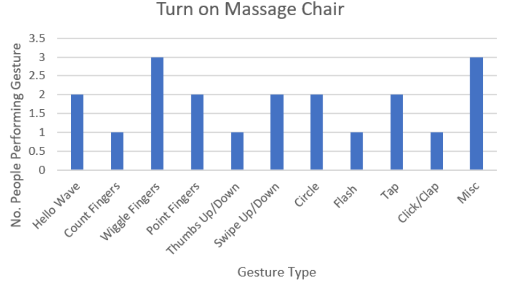
\includegraphics[scale=0.8]{images/massageChair.png}
    \caption{Gestures Elicited for Turning on Massage Chair}
    \label{fig:massageChair}
\end{figure}
\subsubsection{Pulse Duo}: Participants would perform the gesture for pulse twice. This is demonstrated in the videos but unable to be done as well in the raw data.
\subsubsection{Combination}: Most participants performed the first two formats, "wave" and "pulse", sequentially. This is the obvious gesture for this control.
\subsubsection{Hot Stone}: It was hard to find a gesture that was most commonly done as there were 13 different gestures to choose from. "Wiggling fingers" was the one that was performed most often, however. 
\subsubsection{Intensity Level}: The most popular gesture for changing the intensity level was "counting fingers" on one hand with 13 people performing it. 
\subsubsection{Change Colour of Ambient Lighting}: "Swiping left and right" was the most common gesture performed with almost half of the participants doing it for changing colour. The next most common gesture was "counting on individual fingers". 
\subsubsection{Change Brightness Level of Ambient Lighting}: "Swiping up and down" was the most commonly performed gesture for brightness level. However, "swiping up and down" is a commonly used gesture and it would be best if a wide range of gestures were used.
\subsubsection{Mute All Audio}: The most common gesture was "swipe left or right" followed by hold. Swipe left/right also included people swiping quickly in one direction and hold was when they held their hand over the sensor for an extended period. 
\subsubsection{Open Champagne Cooler}: The two most common gestures performed were "swipe up and down" and "drink". The drink gesture involved participants either pretending to "drink" or "pop a cork". This is the most creative gesture and, therefore, most appropriate.
\begin{figure}[!htb]
    \centering
    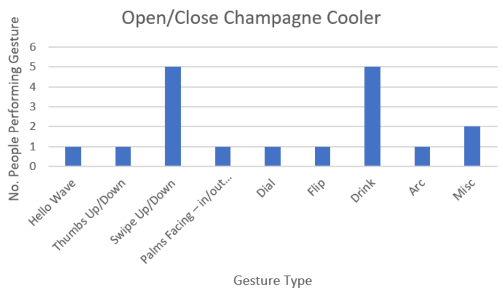
\includegraphics[scale=0.8]{images/champagneCoolerGE.png}
    \caption{Gestures Elicited for Opening Champagne Cooler}
    \label{fig:champagneCoolerGE}
\end{figure}

\section{Follow-Up Gesture Elicitation Survey}
The aim of the follow-up gesture elicitation survey is to give an insight as to what gestures people like and dislike and to find out which gestures are most suitable for the experiment. This was done by creating an online survey using Google Forms (the questions are outlined in Appendix \ref{section:followUpGEQu}) which included videos of every gesture that could be done for a particular control and asking the participant to select their favourite gesture for that control. They were then asked to rate the intuitiveness and if they would prefer to do any other gesture. It was particularly important to ask the participants to rate the intuitiveness of a gesture because, even if it was their favourite gesture, they may not actually find it especially intuitive which may suggest that it would not be the best control to perform a mid-air gesture for. 

Due to the nature of the survey being so similar to the previous one, a selection of new participants were needed. There were 12 participants with 4 being female and 8 being male.

\subsection{Follow-Up Gesture Elicitation Results}
Fortunately, Google Forms processes the results into pie charts and bar graphs. However, it is not possible to do follow up questions, so each question is processed separately. Therefore, the intuitiveness questions needed to be processed separately so that it was possible to see the intuitiveness rating for each gesture rather than how the participants voted overall for intuitiveness (Appendix \ref{section:followUpGEResults}). 

\subsubsection{Adjust Temperature}: 66\% of participants preferred the dial gesture over swiping up and down with 6 either saying they found it very intuitive or intuitive and only 2 participants finding neutral.
\subsubsection{Recline Chair}: 75\% of participants preferred moving their hand on an angle opposed to moving their hand towards their shoulder. However, 2/9 participants who preferred it said they did not find it intuitive. This could suggest that using mid-air gestures for reclining a chair would not be appropriate. However, 5 participants did say it was intuitive and one said it was very intuitive.
\subsubsection{Adjust Footrest}: There was a 50/50 split for whether participants preferred the sweeping motion or moving their fist forwards and backwards. However, only 4 people said it was intuitive or very intuitive while the rest said neutral or not intuitive. This suggests that it may not be appropriate to use mid-air gestures for adjusting the footrest.
\subsubsection{Lumbar Support - Move from Top to Bottom}: The favoured gesture for this control was moving a fist up and down with 75\% of participants voting for it. However, they did not find it overly intuitive with 6/9 participants saying it was neutral.
\subsubsection{Lumbar Support - Pull out and Push In}: The most popular gesture was moving your hand forwards and backwards. However, this does not follow on from the previous selection and, therefore, if we chose hands then it would lack continuity. For both these gestures, people either said it was neutral or intuitive with only one person saying that moving hand was very intuitive. Overall, it would still be appropriate to use fist despite it not being participants’ favourite.
\subsubsection{Head Rest}: Four participants said that swiping hand up and down was their favourite. However, half of them said it was intuitive whereas the other half said it wasn't. This is not an appropriate gesture for this control.\\
Only 2 people thought swiping their fist up and down was the best and 6 thought that pointing their fingers up and down was the best. Most people said that they were neutral towards how intuitive it was with only 2 saying it was intuitive and 1 saying it was not.\\
The results for this control are very mixed but the most appropriate gesture would be pointing fingers.
\subsubsection{Inflate/Deflate Side Bolsters}: Half of the participants chose palms facing as their favourite gesture with it either being neutral or intuitive. Pinch was only chosen by two people but was considered intuitive. However, not enough people chose it to justify choosing this gesture as the most appropriate.
\subsubsection{Adjust Volume}: Eight people chose dial as their favourite gesture with 7/8 participants saying it was very intuitive and 1/8 saying it wasn't intuitive.\\
However, the dial gesture was also chosen to be the favourite gesture for adjusting the temperature. It is not appropriate to have the same gesture used twice for two different controls. Unfortunately, it was the same split for both the controls with 8/12 choosing the dial but more participants said the dial gesture was "very intuitive" for adjusting volume than temperature. This means that it should be volume that uses the dial gesture.\\
An alternative to this could be that, when being used in a car, a passenger selects a button first before gesturing to choose whether they want to adjust volume or temperature so that dial could be used for both.
\subsubsection{Open \& Close Windows}: 75\% of participants preferred the car roller gesture with 7/9 saying it was very intuitive and 2/9 saying it was intuitive. This is undoubtedly the most appropriate gesture.
\subsubsection{Turn Massage Chair On \& Off}: 75\% of participants preferred wiggling their fingers to turn on the massage chair. The intuitiveness was varied but no one said it was not intuitive.
The other two options that were chosen were circle and tap.
\subsubsection{Wave}: Participants did not get to choose their favourite as most people from the previous survey did this gesture. However, they were able to rate the intuitiveness and no one thought it was not intuitive.
\subsubsection{Pulse}: 66.7\% of participants chose the Flash gesture as their favourite with 6/8 saying it was intuitive or very intuitive. However, two participants did say it wasn't intuitive. Three participants chose Tap as their favourite gesture and only one person chose Punch as being their favourite gesture.\\
Overall, it still makes the most sense to choose flash as the most appropriate gesture.
\subsubsection{Pulse Duo}: There was a 50/50 split between Flash and Tap for the pulse duo format. However, more people said that Flash was intuitive and very intuitive than Tap.
\subsubsection{Combination}: Combination format had mixed reviews from people with two people saying it wasn't intuitive.
\subsubsection{Hot Stone}: Most participants said that hold was their favourite gesture with 5/12 saying that. However, there are very mixed ratings for it with 2 votes for neutral and 1 vote each for very intuitive, intuitive and not intuitive.
3 people picked flash as their favourite gesture but it is the most appropriate gesture for pulse and pulse duo format so it would not work in this scenario. Furthermore, one person did vote that it was not intuitive at all.
3 people picked wiggling fingers as their favourite gesture, but this is the gesture that was favoured for turning on the massage chair.
Only one person chose moving their fist up and down and they said it was intuitive.
Overall, it makes most sense to choose Hold as the most appropriate gesture for hot stone format due to a process of elimination and the fact that it was chosen by the most people.
\subsubsection{Intensity Level}: Most people thought that counting on your fingers to change the intensity level was the most appropriate gesture with 9/12 people saying this. No one voted that it wasn't intuitive.
\subsubsection{Change Colour of Ambient Lighting}: Swiping Left and Right had a mixture of answers but only one person said it was not intuitive. Therefore, it is still appropriate for this control.
\subsubsection{Change Brightness Level of Ambient Lighting}: Half of the participants chose swiping up and down as their preferred gesture for adjusting the brightness level. However, 2 people did say that it wasn't intuitive.\\
Due to counting fingers and flash being chosen as appropriate gestures for other controls, swiping up and down is the best option.
\subsubsection{Mute All Audio}: The preferred gesture for muting audio was the cross gesture with all 6 participants who chose it saying it was very intuitive.\\
Hold and swiping left/right were also chosen as favourites and were said to be intuitive or very intuitive.
\subsubsection{Open Champagne Cooler}: The drinking gesture was the favourite gesture for this control where 10/12 participants chose it and seven out of those ten said it was very appropriate.
This is the obvious choice for opening and closing the champagne cooler.

\subsection{Issues}
The follow-up survey was necessary as the previous one elicited a vast set of gestures to choose from. However, when it was decided that it would be an online survey rather than a face to face interview, Google Forms was chosen to be used. This proved to be quite difficult to work with as it was not possible to upload videos from a computer or even from a Google Drive. Each gesture was filmed individually and then had to be uploaded to YouTube for the Google Form to display them. The videos took hours to upload and the browser would not allow them to be changed to unlisted so that had to be done on the app for each individual gesture. This meant that the follow-up survey was released much later than originally planned which was already a problem due to having difficulty finding participants who had not performed in the previous survey.

\section{Conclusions Drawn}
\label{section:conclusions}
The first gesture elicitation survey allowed for many different gestures to be introduced. However, due to the vast amount of them, it was difficult to judge which gestures were most appropriate for a certain control. 

The follow-up gesture elicitation survey was made so that participants could pick which gestures they found most appropriate for each control. This led to more conclusive results which could be analysed. Some of the controls, such as reclining the massage chair, had multiple gestures that were similar to each other for the different features. 

Overall, there were enough gestures for each control that was provided so it would be easy to create a set of controls with unique gestures.


%==================================================================================================================================
\chapter{Design}
\section{Gesture Set}
In order to begin creating an experiment for users to participate in, a gesture set had to be created. This was done by reviewing the conclusions drawn from the gesture elicitation survey and choosing a mixture of controls and gestures that are unique, recognisable by the Leap Motion Sensor and easy for a user to perform. 

Looking at Section \ref{section:conclusions}, it was clear that the reclining chair controls were not going to be appropriate as they included too many similar gestures to each other. Therefore, it made more sense for the massage chair features to be chosen to gesture for. A feature of the massage chair not included was the combination programme. It seemed unnecessary to include it as it incorporated two of the previous gestures performed sequentially. This would only give five different controls to be performed so five more were chosen so there was a wide variety of options. 

Opening the champagne cooler was chosen due to its uniqueness - this is not a feature many cars have. Changing the colour and brightness of the ambient lighting was chosen for the same reason. However, adjusting the temperature and volume in the car was chosen to ensure there were some familiar controls for the users. 

In order to work out what gestures should be chosen for each control a comprehensive catalogue, provided by the \cite{leapmotion_api_nodate} API reference, of all the gestures and motions that can be performed was consulted. This helped to eliminate certain gestures that could not be implemented such as wiggling fingers or the sea wave, gestures with very small increments that the Leap Motion wasn't sensitive enough to recognise.

\begin{figure}[!htb]
    \centering
    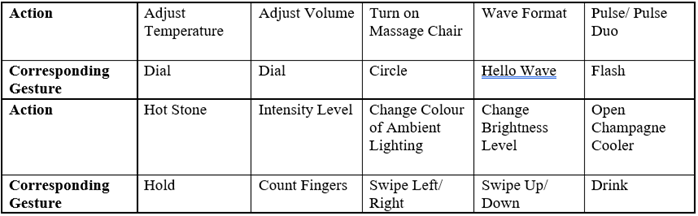
\includegraphics[scale = 0.8]{images/gestureDesign.png}
    \caption{Gesture Set}
    \label{fig:gestureDesign}
\end{figure}

Even though the wave programme had a clear favourite gesture - the "sea wave" motion - the second favourite gesture -the hello wave - was selected. This was due to the simplicity of waving your hand and the fact it is a commonly used gesture.

Replacing wiggling fingers for turning on the massage chair was harder as there were multiple different gestures to choose from. However, circle was chosen as it was part of the built in gestures that Leap Motion has. It also hadn't been chosen for any other control and, therefore, unique.

The final gesture set is shown in Table \ref{fig:gestureDesign}.

\section{Wireframes}
For the wireframes, the designs were kept simple. This was to ensure that, while taking part in the experiment, participants would not need any guidance as to what the screen is indicating.

Balsamiq was used to create the wireframes as it is a tool that is designed for creating digital wireframes of applications or websites. It has many built in icons and shapes so that it is easy to create wireframes without them looking messy or cluttered.

The wireframes that were chosen to be created were based on the gesture set created previously. By creating the gesture set first, it meant that no wireframes were created that were unnecessary.

The wireframes were made to represent the 10” touchscreens that are provided in the backseat of a Range Rover. They are loosely based off the graphics that Range Rover already provide. However, some needed a bit more detail and creativity added so that it was obvious to the participant what they were looking at. Furthermore, the passengers would be using mid-air gestures to make selections rather than just selecting using a touchscreen, so the feedback did not need to be so obvious.

The first wireframe that was created was the ambient lighting function, shown in figure \ref{fig:ambientLighting}, which displayed the current colour as the main body of the screen. The ten colour options were at the bottom of the screen to help passengers decide which direction they would like to swipe. There was a slider at the top to adjust the brightness, but this was removed during implementation so that the user could receive feedback for each gesture independent of each other.

\begin{figure}[!htb]
    \centering
    
\includegraphics[scale = 0.5]{images/ambientLighting.png}
    \caption{Ambient Lighting Wireframe}
    \label{fig:ambientLighting}
\end{figure}

The next wireframe that was created was for the temperature adjustment function which was a simple circle in the middle of the screen with a dial. As the temperature is adjusting the dial will move accordingly and as the temperature moves from cold to hot, the colour around the circle will change from blue to red and vice versa. This design was also used for adjusting the volume, but the circle colour was removed.

The design for turning the massage chair on was also very similar to the previous wireframe but instead had a power symbol in the middle of the circle and would glow red when the massage chair was turned off and green when it was turned on.
The wave programme was designed so that, when the user waved, there would be waves shown on the screen.
The Hot Stone programme wireframe had “warm coloured” balls on the screen to represent hot stones. The Pulse and Pulse Duo format were designed separately as one circle on the screen for pulse and two on the screen for pulse duo.
A wireframe for combination was made even though there was no plan to implement it. But it had waves and a pulse circle on it. 

The wireframes for the massage chair programmes had a slider bar at the top of the screen. However, it was later decided that it was too similar to the ambient lighting and was changed to have the numbers 1-5 on the screen depending on how many fingers were held up.

Finally, the champagnes wireframe (Figure \ref{fig:champagne}) was designed to have a champagne glass in the middle surrounded by stars. When the champagne cooler is “opened” the stars will spin and it’ll look like there is fizz coming out of the glass.

\begin{figure}[!htb]
    \centering
    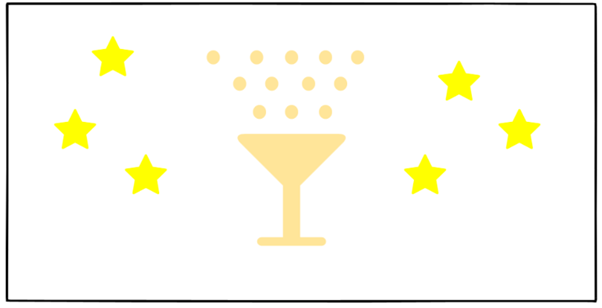
\includegraphics[scale = 0.5]{images/champagneCooler.png}
    \caption{Open Champagne Cooler Wireframe}
    \label{fig:champagne}
\end{figure}

All of the wireframes created can be seen in Appendix \ref{section:wireframes}

\section{Experiment}
\label{section:desExperiment}
It was decided that all of the gestures should be performed independently of each other. This meant that, instead of users doing one big experiment, they would participate in 10 smaller ones that would allow assessment of how well each gesture was performed. These would be set up by the evaluator and it would be controlled from the command line. This ensures that each participant has the best chance of performing a gesture correctly as there is no way for the Leap Motion sensor to confuse it with another one. Another option could have been to comment out the irrelevant code for each experiment to avoid code duplication. However, this was deemed to be overly wasteful of time when the experiment takes place.


%==================================================================================================================================
\chapter{Implementation}
\section{GitHub}
GitHub was used consistently throughout the project. It was used as an online repository to store all important files related to the project, ensuring that all the code was backed up and would not be lost if there were any issues locally. However, it was also used as a form of version control. Version control was not needed extensively for this project as once a gesture was implemented and tested, it rarely needed to be revised. However, it was a faster way of backing up the data compared to other methods. The repository can be found here: \url{https://github.com/catrionamurphy/midAirGestures}

However, GitHub was also a useful tool due to it having a "Wiki" section. This wiki section allowed for any research notes, rough analysis and meeting minutes to be organised into separate pages for easy access. These could  be edited to have subheadings so that all the pages were in the correct order, regardless of when they were created. 

\begin{figure}[!htb]
    \centering
    \begin{subfigure}[b]{0.3\textwidth}
        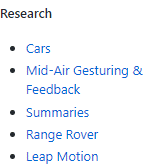
\includegraphics[scale = 0.8]{images/wiki2.png}
    \end{subfigure}
    \begin{subfigure}[b]{0.2\textwidth}
        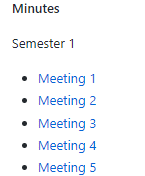
\includegraphics[scale = 0.8]{images/wiki3.png}
    \end{subfigure}
    \caption{GitHub Wiki Sidebar}
    \label{fig:wiki}
\end{figure}

\section{Leap Motion}
\subsection{Initial Issues}
Originally, the wrong Software Development Kit (SDK) was downloaded as there were many different types and the documentation was unclear on which SDK should be used for Python. It was discovered that, for Python, the Orion SDK was necessary. 

The documentation did not specify which version of Python should be used for the version which was downloaded. It was discovered that the wrong version of Python was installed on the machine being used. This was adjusted by uninstalling Python 3 and Anaconda Studio, and installing Python 2.7. The "Hello, World" tutorial was then able to be followed and it ran successfully. 

These issues caused a slight delay in starting the implementation but once rectified, there were no further problems.

\subsection{Learning the Basics}
Having no prior experience of using a Leap Motion Sensor or any other form of gesture sensors, it was important to learn how the Leap Motion detected fingers, hands and their movements. To do so, the diagnostic visualiser of the leap motion was used. The diagnostic visualiser allows a user to try out different hand poses and movements and see how their hand is represented by the Leap Motion software. Figure \ref{fig:diagnosticVisualiser} shows three different hand poses with Figure \ref{fig:drinkGesture} showing the hand and finger placement that participants in the experiment will need replicate for opening the champagne cooler. 

The visualiser was not always completely accurate and would sometimes mistake how many fingers were up or down. This further confirmed that a 'wiggling fingers' gesture would have been unsuitable as it became clear that the sensor would not have been able to recognise it. Additionally, it shows that if gestures do need individual fingers to be used throughout, then it may be better for them to be a static gesture. A static gesture is one which requires no movement. All non-static gestures in the created gesture set were designed so that finger position did not change.
The gesture for changing the intensity level of the massage chair could potentially have a problem due to it having multiple fingers held up at a time but the participants will be made aware that they should perform this gesture slowly so that the Leap Motion will pick their gesture up correctly.

\begin{figure}[!htb]
    \centering
    \begin{subfigure}[b]{0.45\textwidth}
        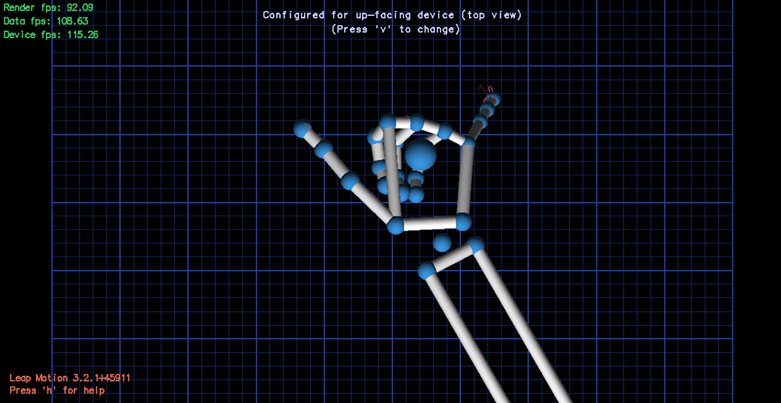
\includegraphics[scale = 0.22]{images/drinkGesture.png}
        \caption{Diagnostic Visualiser showing the Drink Gesture}
        \label{fig:drinkGesture}
    \end{subfigure}
    \begin{subfigure}[b]{0.45\textwidth}
        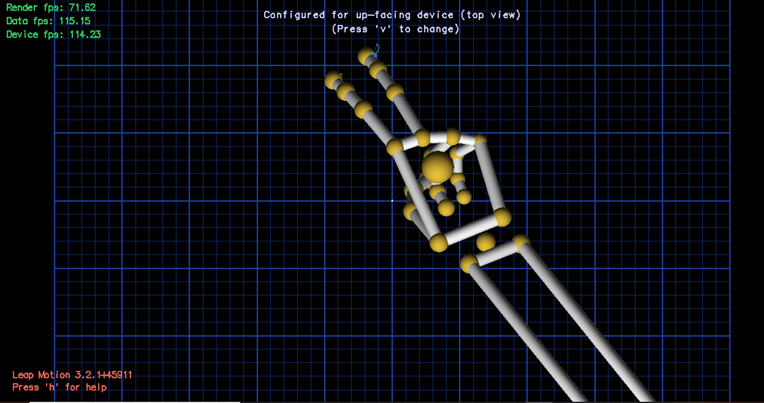
\includegraphics[scale = 0.22]{images/twoFingers.png}
        \caption{Diagnostic Visualiser showing Two Fingers Up}
        \label{fig:twoFingers}
    \end{subfigure}
    \begin{subfigure}[b]{0.45\textwidth}
        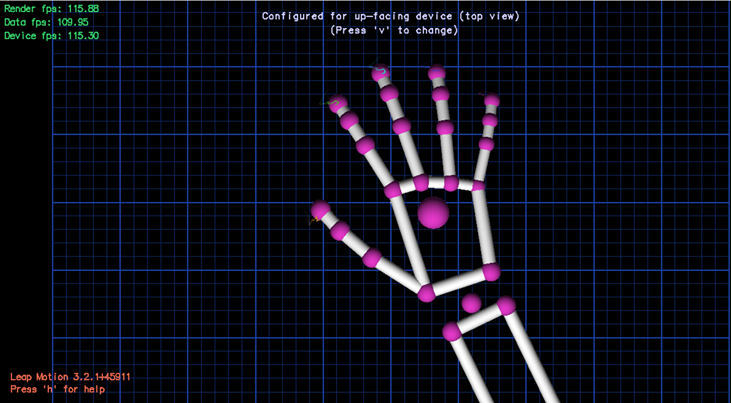
\includegraphics[scale = 0.22]{images/fullHand.png}
        \caption{Diagnostic Visualiser showing Full Hand}
        \label{fig:fullHand}
    \end{subfigure}
    \caption{Leap Motion Diagnostic Visualiser}
    \label{fig:diagnosticVisualiser}
\end{figure}

In order to gain an understanding into how to program the Leap Motion, an online tutorial was followed. The \cite{Coding_Basics_2014} Leap Motion Tutorial in Python was a very useful tool in understanding how different body parts and gestures can be recognised. By following this tutorial a Python Program was created that had every aspect  needed for the implementation. 

Another important tool in learning how to program the Leap Motion was the online API Reference (\cite{leapmotion_api_nodate}). This was especially useful in providing a deeper understanding of how certain attributes or methods worked. 

\subsection{Implementing the experiment}
As mentioned in the design section (Section \ref{section:desExperiment}), each experiment was developed independently of each other. However, they did follow a similar structure. Each experiment code contained a 'Listener' class. This class would be 'listening' for a gesture to be performed and it would store all the necessary variables. There were five main functions that were contained within a class: on\_init, on\_connect, on\_disconnect, on\_exit and on\_frame. These all had 'self' and 'controller' passed into them, with controller being the Leap Motion Sensor. These functions recognise when the Leap Motion sensor was initialised, connected, disconnected and exited, and their only function is to print to the command line what is happening, for example, if a circle gesture was performed, then "circle" would be printed on screen. The last function was called when the Leap Motion sensed an object and tried to start recognising what the user was doing. 

The listener class was called from a main function which simply set up the controller and the listener. The on\_frame function was the most important class to differentiate between the experiments as that is where the gesture recognition is programmed. Within this function, it could be determined if there was a hand in front of the sensor or if there was a gesture being performed. For example, there are four different gestures which are built into the Leap Motion sensors so when the Leap Motion is connected, it can automatically detect if there is a gesture being performed if it's been enabled. 

\subsubsection{Massage Chair On \& Off}: This was one of the more straightforward gestures to implement as the circle gesture is built into the Leap Motion software. For it to turn on and off, the direction of the gesture had to be determined. In order to debug the code, the direction of the circular motion was printed to the command line as there was no GUI yet. This helped to determine whether the Leap Motion was detecting the gesture properly. In doing so, it was noticed that it wasn't always picking up circles fully. To combat this, the progress of the circle was adjusted so that the leap motion didn't have to detect a full circle but only one that was 4/5 of a circle. This would then print if the massage chair was turned on or off, depending on whether the circle was clockwise or anticlockwise. 

\subsubsection{Ambient Lighting Colour \& Brightness} The Leap Motion also had the swipe gesture built into its software. However, it was unreliable and did not detect swipes particularly accurately. A Glasgow University lecturer and advisor, Dr. Euan Freeman, gave a useful insight into the swipe gesture and provided his code that had been used to implement the swipe gesture for a Microsoft Kinect. This involved finding the starting and ending coordinates of the swipe motion and finding the greatest difference in the axes. For example, if the x-axis had the greatest difference in coordinates, then the user would be swiping from left to right and if the z-axis had the greatest difference, the user was swiping up and down. In order to determine when a swipe starts and finishes a list was created to store all the frames from when a users hand is "on frame". Once the list exceeded 200, the final direction could be determined and the list was cleared. If the hand was taken away from the frame, then the frame count list would stop adding frames and wait until a user brought their hand back into the frame.

\subsubsection{Intensity Level}: The counting fingers gesture was simple to implement. The Leap Motion has the ability to tell how many fingers are extended. Therefore if there were two fingers held up, then that would indicate two extended fingers. The .extended() method, as shown in Figure \ref{fig:extendedFingers}, creates a list of the finger types that are extended and by taking the length of this list the number of fingers held up can be determined.

\begin{figure}[!htb]
    \centering
    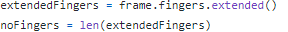
\includegraphics[scale = 0.9]{images/extendedFingers.png}
    \caption{Code Required to Determine How Many Fingers are Held Up}
    \label{fig:extendedFingers}
\end{figure}

\subsubsection{Wave Format}: The gesture for the wave format makes use of the circle gesture and the extended finger method. For this to work, the user must have four or five fingers extended and wave slowly in an arc motion so that the progress of the circle is less than one i.e. the user does not gesture a full circle but only a segment of one.  

\subsubsection{Pulse \& Pulse Duo}: The flash gesture was initially meant to be implemented with the user having four or five fingers extended and then zero. Unfortunately, the Leap Motion sensor was not able to capture this hand movement particularly well especially when trying to track the number of fingers. A new approach had to be taken where the hand's "grab strength" was involved. If a users grab strength was 1, then it meant they had their hand in a tight ball. If it was less than one then it meant their fist was open. In order to track this as a flash gesture, a frame list was created but instead of tracking all of the frames, it tracked the grab strength. Once the list length reached 200, each item was compared to the following item. If the first item was equal to 1 and the following was less than one, then a flash gesture had been accomplished. The number of flash gestures performed within the list was tracked and if there was one, then the user had performed flash and if it was two, then the user had performed pulse duo. 

\subsubsection{Temperature \& Volume}: Temperature and Volume both involved the same dial gesture. This was done similarly to the swipe gesture but, instead of using the x or z coordinate, yaw was used. Yaw is the angle around the y-axis which is shown in Figure \ref{fig:yaw}. The dial gesture also makes use of there being an available list of frames and depending on the difference between the starting yaw angle and ending yaw angle, the temperature or volume would adjust. For example, if the starting angle was smaller than the end angle the volume/temperature would increase.

\begin{figure}[!htb]
    \centering
    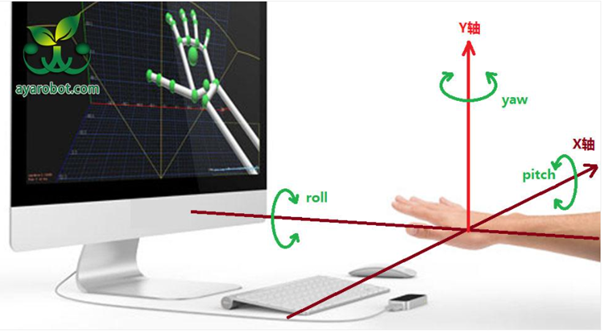
\includegraphics[scale = 0.5]{images/yaw.png}
    \caption{Pitch, Yaw \& Roll on a Leap Motion Device (\cite{ProgrammerSought})}
    \label{fig:yaw}
\end{figure}

\subsubsection{Open Champagne Cooler}: An important aspect of the drink gesture was that the pinky finger and thumb had to be extended as this represented holding a drink. This gesture also used the yaw angle to determine if the user was performing the arc movement from their side to roughly their mouth. Finding the right angles to use required a lot of trial and error but, in the end, the starting angle should be greater than 40 and the ending angle should be less than 10.

\subsubsection{Hot Stone Format}: The final gesture to implement was simply for the user to hold their hand still in front of the sensor. This was done by using the same structure as the swipe gesture. However, it was not necessary to find what axis the user was moving the most on as they were to hold their hands as still as possible. The differences of all three axes starting and ending coordinates had to be less than 5 for it to be considered that someone's hand was being held still.

\section{PyGame}
PyGame was used to create a graphical user interface (GUI) which was integrated with the Leap Motion Code. These interfaces were based on the wireframes created previously and had a basic, minimalist design so the screen was not too cluttered. 

\subsection{Learning the Basics}
Similarly to the Leap Motion software, learning the basics was an integral part of the development of the GUIs. \cite{Nerd_Paradise} Beginner's tutorial for implementing PyGame was used to learn the basics of drawing shapes and moving them around the screen. This also included setting up the window to open and what happens when it is closed.
Further research was done on how to incorporate "sprites" into the programs. A sprite in PyGame is any graphic that can be moved around on the screen and is interactive. There are classes for different sprites and functions can be defined within these classes to perform actions. The first function within the sprite class is to initialise the sprite. This includes its size and shape and most importantly, if it is necessary for it's background to be transparent against the window, its 'colorkey' is set to match the window.

\subsection{Implementing the User Interfaces}
Having gained experience in implementing small games in PyGame, the next step was to find the correct graphics for each user interface. \cite{OpenGameArt.org} is an open source website that specialises in providing graphics that are perfect for animated gaming systems. Although the aim of this project was not to make a game, the interface will involve movement of objects and it is necessary for them to be as basic and as clear as possible. Once the appropriate graphics were found and stored correctly, the interfaces were created. 

The first interface that was created was for changing the ambient lighting. This required 10 different coloured blocks at the bottom of the window and a large block in the centre of the screen. There was no interactivity involved with this interface as it had yet to be integrated with the Leap Motion software for swiping left and right. Adjusting the brightness did involve the use of a sprite to be the circle slider. This was set up with all the appropriate variables.

Turning the Massage Chair On \& Off required some additional tutorial guidance to complete as it required for a partially drawn circle to represent the power button (Figure \ref{fig:powerButton}). \cite{Conrad} explained in depth the best way to draw the circle with the correct starting and end points. This tutorial was followed and then a red and a green circle which were slightly larger than the power button were drawn to indicate either off or on. 

\begin{figure}[!htb]
    \centering
    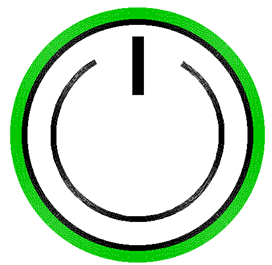
\includegraphics[scale = 0.5]{images/powerButton.png}
    \caption{Partially Drawn Circle within Massage Chair Power Button}
    \label{fig:powerButton}
\end{figure}

The Wave function was difficult to implement as it required the screen to look as though there was a wave moving. \cite{Eastwood_2015} demonstrated how to animate a sine wave using PyGame. This was adapted so that there were multiple sine waves on the screen. They were coloured different shades of blue. Figure \ref{fig:waveGUI} shows what the final GUI looked like for the Wave Format.

\begin{figure}[!htb]
    \centering
    \begin{subfigure}[b]{0.45\textwidth}
        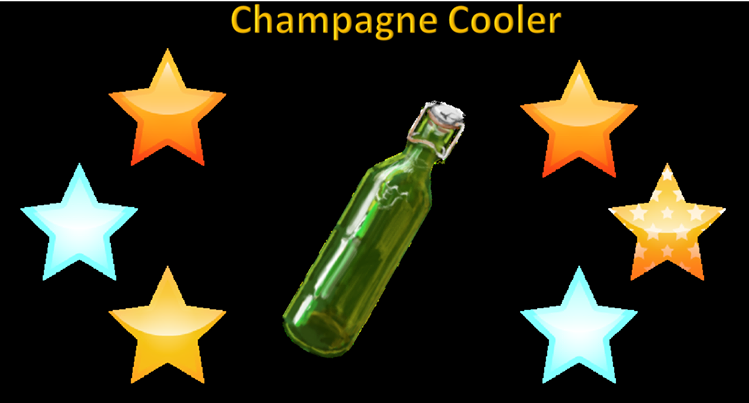
\includegraphics[scale = 0.22]{images/champagneGUI.png}
        \caption{Opening Champagne Cooler GUI}
        \label{fig:champGUI}
    \end{subfigure}
    \begin{subfigure}[b]{0.45\textwidth}
        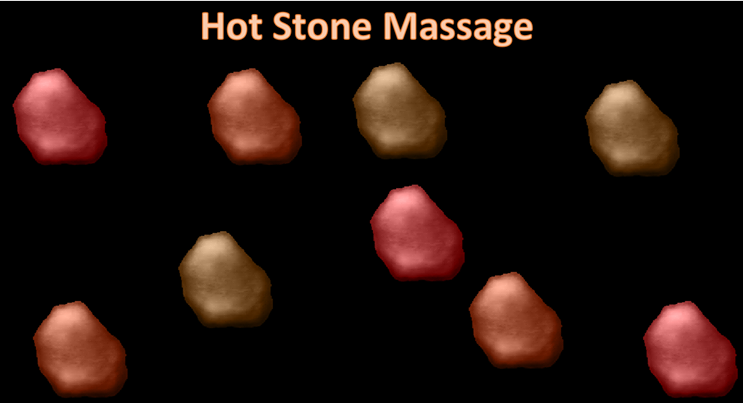
\includegraphics[scale = 0.22]{images/hotStoneGUI.png}
        \caption{Hot Stone Massage GUI}
        \label{fig:stoneGUI}
    \end{subfigure}
    \begin{subfigure}[b]{0.45\textwidth}
        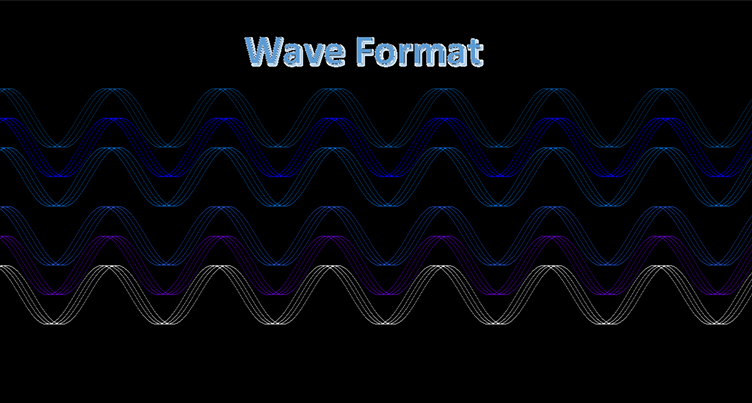
\includegraphics[scale = 0.22]{images/waveFormat.png}
        \caption{Wave Format GUI}
        \label{fig:waveGUI}
    \end{subfigure}
    \caption{PyGame Graphical User Interfaces}
    \label{fig:pygameGUI}
\end{figure}

\cite{Bradfield_2016} created a tutorial on an asteroid shooting game where the rocks moved and spun at the same time. The spinning movement was incorporated into the champagne cooler as it was necessary for the stars to spin. In order for this to work, the stars were initialised as sprites and the speed in which they were to rotate at was initialised within the class along with a variable that measures how many degrees the sprite should have been rotated by. A timer is initialised as well to ensure that enough time has passed before the sprite can be changed again.\\
A sprite can be updated and within this function another function is called which will make it rotate. It is important to note that, if a copy of the sprite is not made before rotating, then the pixels will not line up on each rotation. Each time the sprite is updated and rotate function is called, the variable that measures the rotation of the sprite is updated. Finally, so the sprite spins in the one place, the centre is updated to be the same every time. There were six stars that belonged to this sprite class and they were spaced evenly on each side of a champagne bottle graphic.

The hot stone format also used the spinning movement, but with rocks that were coloured red, orange and gold.

Pulse and Pulse Duo was an easy interface to implement as it required the large orbs (sprites) to show on the screen when the gesture was performed. However, since it was not integrated with Leap Motion, there was no interactivity.

Temperature, volume and intensity level all required the same sprite set up as it was only different numbers that appeared on the screen. This relies on the Leap Motion interaction so they were very basic and simply had the relevant graphics initialised as sprites. Temperature and volume both had a circle drawn around their numbers as well with temperature also having three different coloured circles around the first circle

The final designs for three of the experiments can be seen in Figure \ref{fig:pygameGUI}.
\section{Final Product}
The final product consisted of 10 separate Python files which incorporated both the Leap Motion and PyGame code. It was easier to incorporate these together for some experiments over others. However, they all started by importing Leap and PyGame. Furthermore, within the main function of the Leap Code, the window size and colour was defined and any graphics that were required were initialised and the Leap listener was called while the PyGame window was running.

\subsubsection{Massage Chair On \& Off}: Whenever a clockwise circle was gestured, a green circle was drawn around the power button, and whenever an anticlockwise gesture was drawn, a red circle was drawn around the power button.

\subsubsection{Ambient Lighting Colour \& Brightness}: Changing the colour of the ambient lighting was simple as a list was created with all the possible colours and a counter was created to keep track of what colour the user was on. When a user swiped in either direction, the counter would adjust accordingly and a rectangle would be drawn in the middle of the screen. The rectangle colour would be determined by whichever colour in the list corresponds to the counter. Adjusting the brightness included a sprite class which allowed a circle to be moved forward three times and back three times. If a user performed four swipes up in a row, then the circle would stop after the third time.

\subsubsection{Intensity Level}: For the number of fingers being held up by a user, the sprite class would be called with that number and the corresponding image would be displayed in the middle of the screen.

\subsubsection{Temperature \& Volume}: For temperature, the sprite class is called once the temperature has been determined. This changes the number shown on screen and the colour of the circle. Volume works the same way except there is no coloured circle.

\subsubsection{Wave Format}: Within the listener class, whenever a wave was detected, a new function called 'wave' was called six times. This function draws the sine waves across the window. 
\subsubsection{Pulse \& Pulse Duo}: When a pulse was detected within the listener class, the sprite class would be updated and it would check if the gesture was a pulse and only one orb would be shown in the middle of the screen and if the gesture was two pulses, then two orbs would be shown on screen.

\subsubsection{Open Champagne Cooler}: When a drinking gesture is recognised the sprite class is called and the six stars start spinning around the bottle.

\subsubsection{Hot Stone Format}: If the sensor detected a hold gesture, then the sprite class would be called and the rocks would start rotating.

\subsubsection{Adjustments for Gesturing to Side}: The brightness level and champagne cooler experiments had to be adjusted for performing the gesture when the sensor was on the centre console. This simply required the axis to be changed from z to y for the brightness level and the angle to be changed from yaw to roll for opening the champagne cooler.

%==================================================================================================================================
\chapter{Experiment and Evaluation}
\section{Experiment Aim}
The aim of the experiment was to learn about what gestures could be performed most effectively by passengers in the backseat of a car. To do so, participants were asked to sit in the back seat of a car and perform a series of gestures with a motion sensor facing them or to their side. They were able to view a laptop screen which provided feedback as to whether they were performing the gestures correctly or not. Following this, they were asked to fill out a NASA Task Load Index survey to measure their “workload” after performing gestures facing forward and after performing gestures to their side. Following the experiment, they were asked to fill out a questionnaire which asked them their general opinions on the survey including questions about the feedback used, the gestures themselves and where they sat in the car (Appendix \ref{section:expSurvey}). 

\section{Experiment Set-Up}
The experiment had to be done in a car. Unfortunately, a Range Rover could not be accessed, so a Ford Focus was used. Inside the car, the sensor was placed between the head rest and the seat in front of the participant. Participants could choose which seat they wanted to sit in. A laptop sat in the centre console between the front two seats with the screen facing the participant so they could see the given feedback (\ref{fig:setUp1}). When the participant had finished gesturing in front, the sensor was moved to be positioned in the centre seat next to them (\ref{fig:setUp2}). If this had been in a Range Rover, there would have been a back seat centre console, but with the car available to use, there was only a middle seat. This set-up was kept consistent between all 8 participants.

\begin{figure}[!htb]
    \centering
    \begin{subfigure}[b]{0.45\textwidth}
        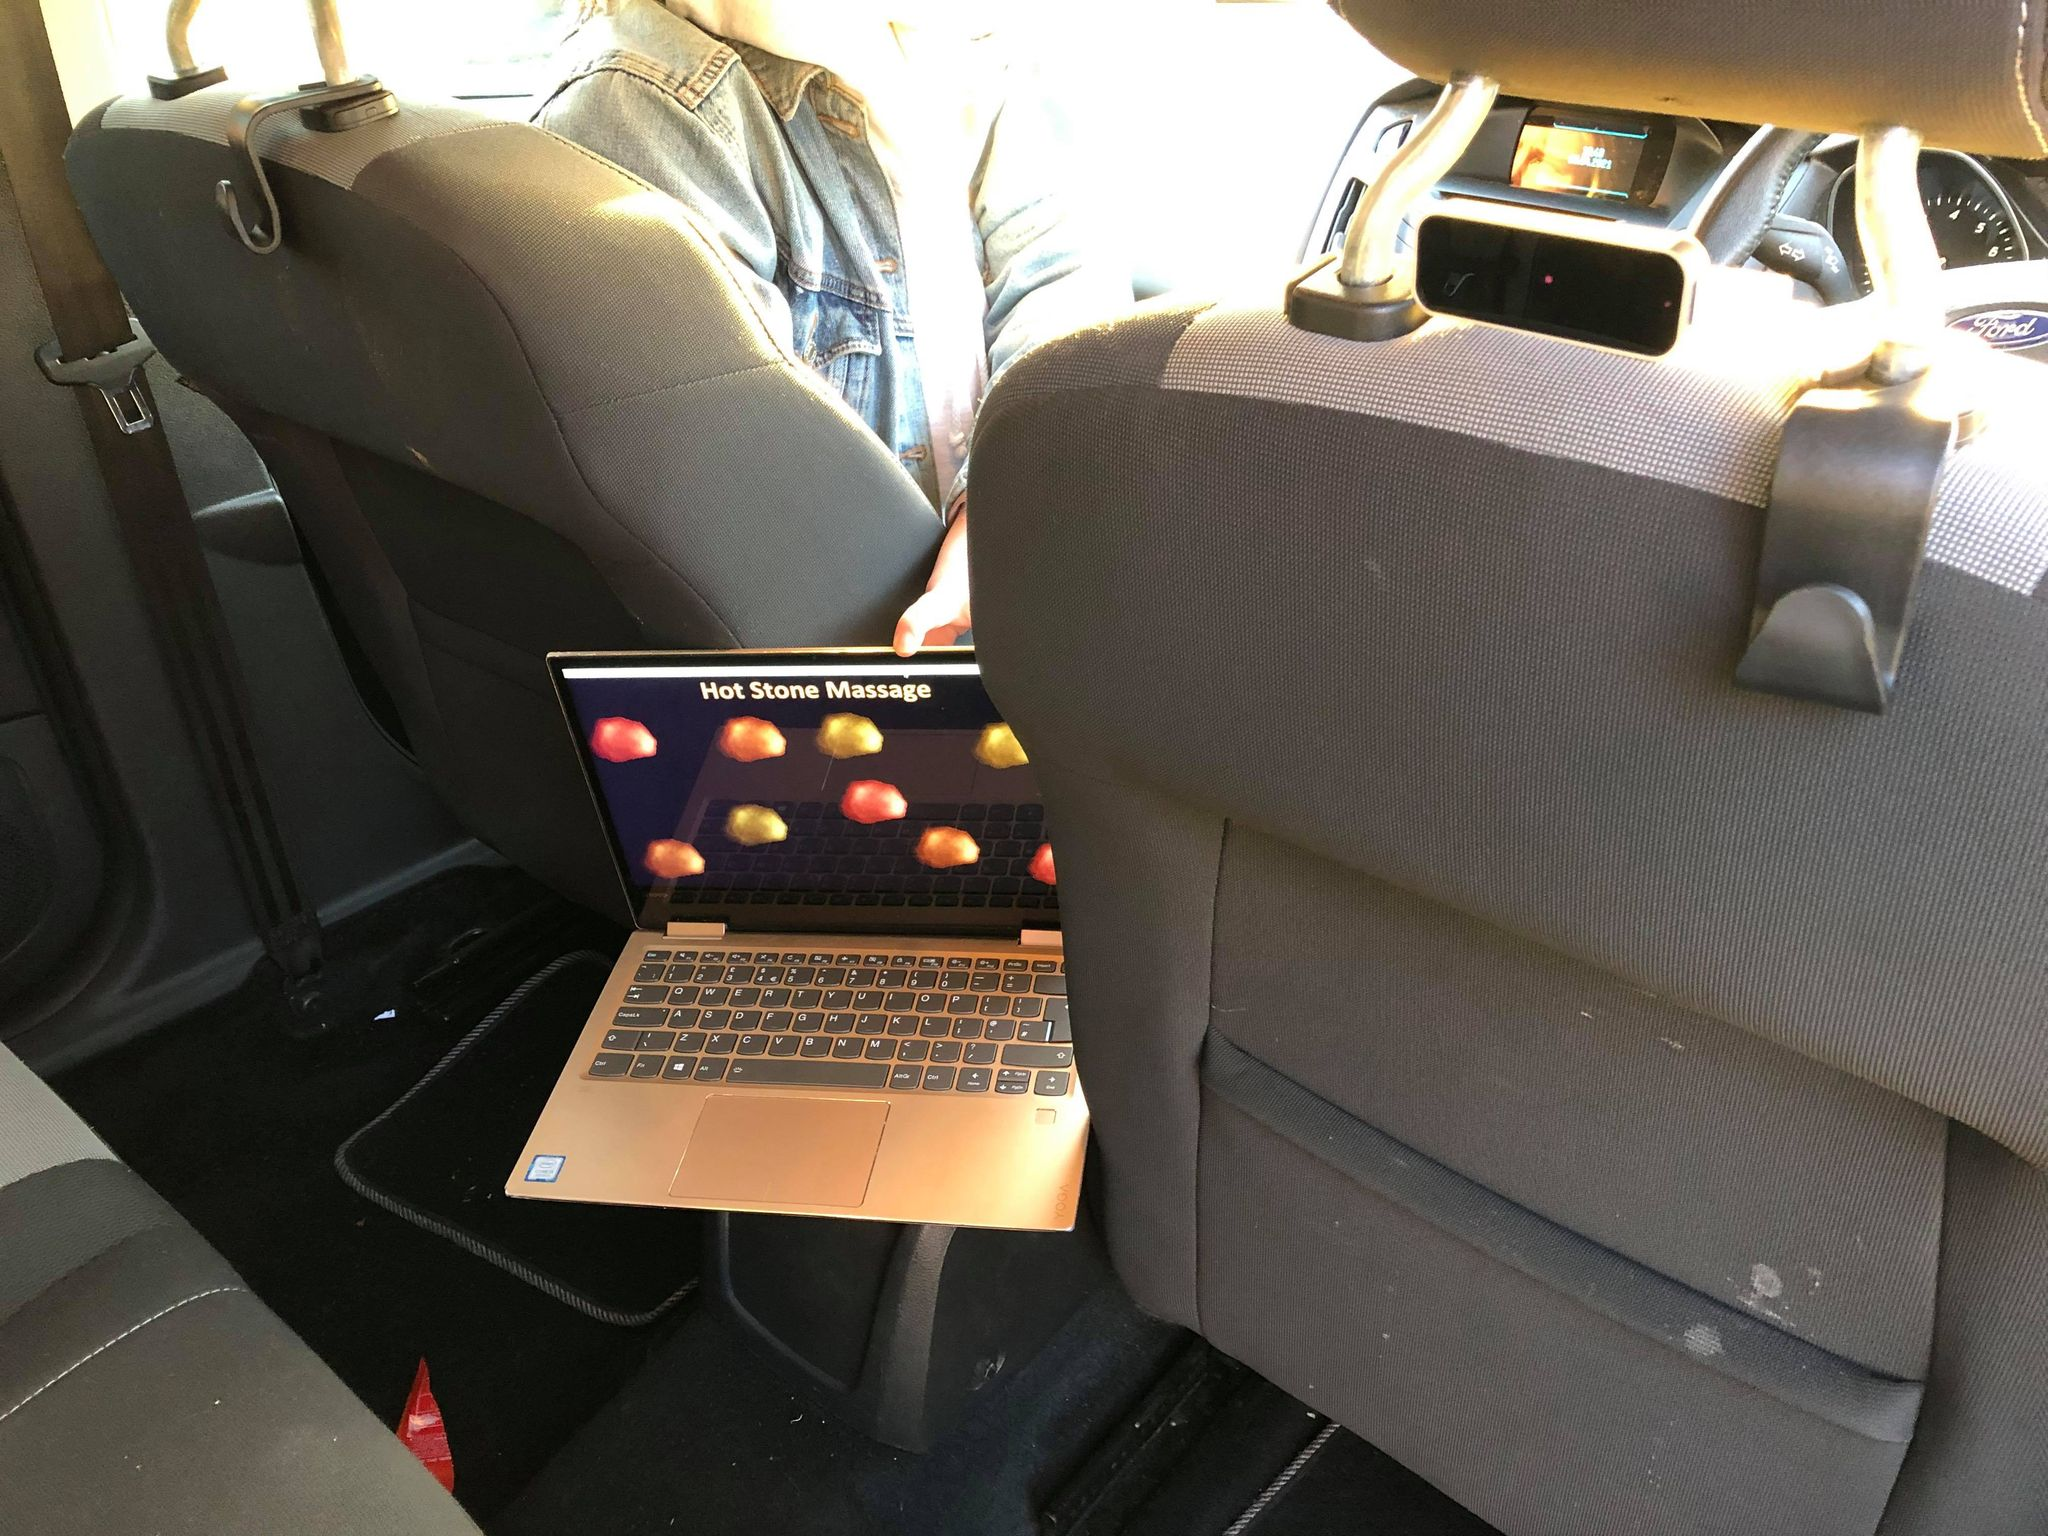
\includegraphics[scale = 0.08]{images/experimentSetUp1.jpg}
        \caption{Sensor Facing Participant}
        \label{fig:setUp1}
    \end{subfigure}
    \begin{subfigure}[b]{0.45\textwidth}
        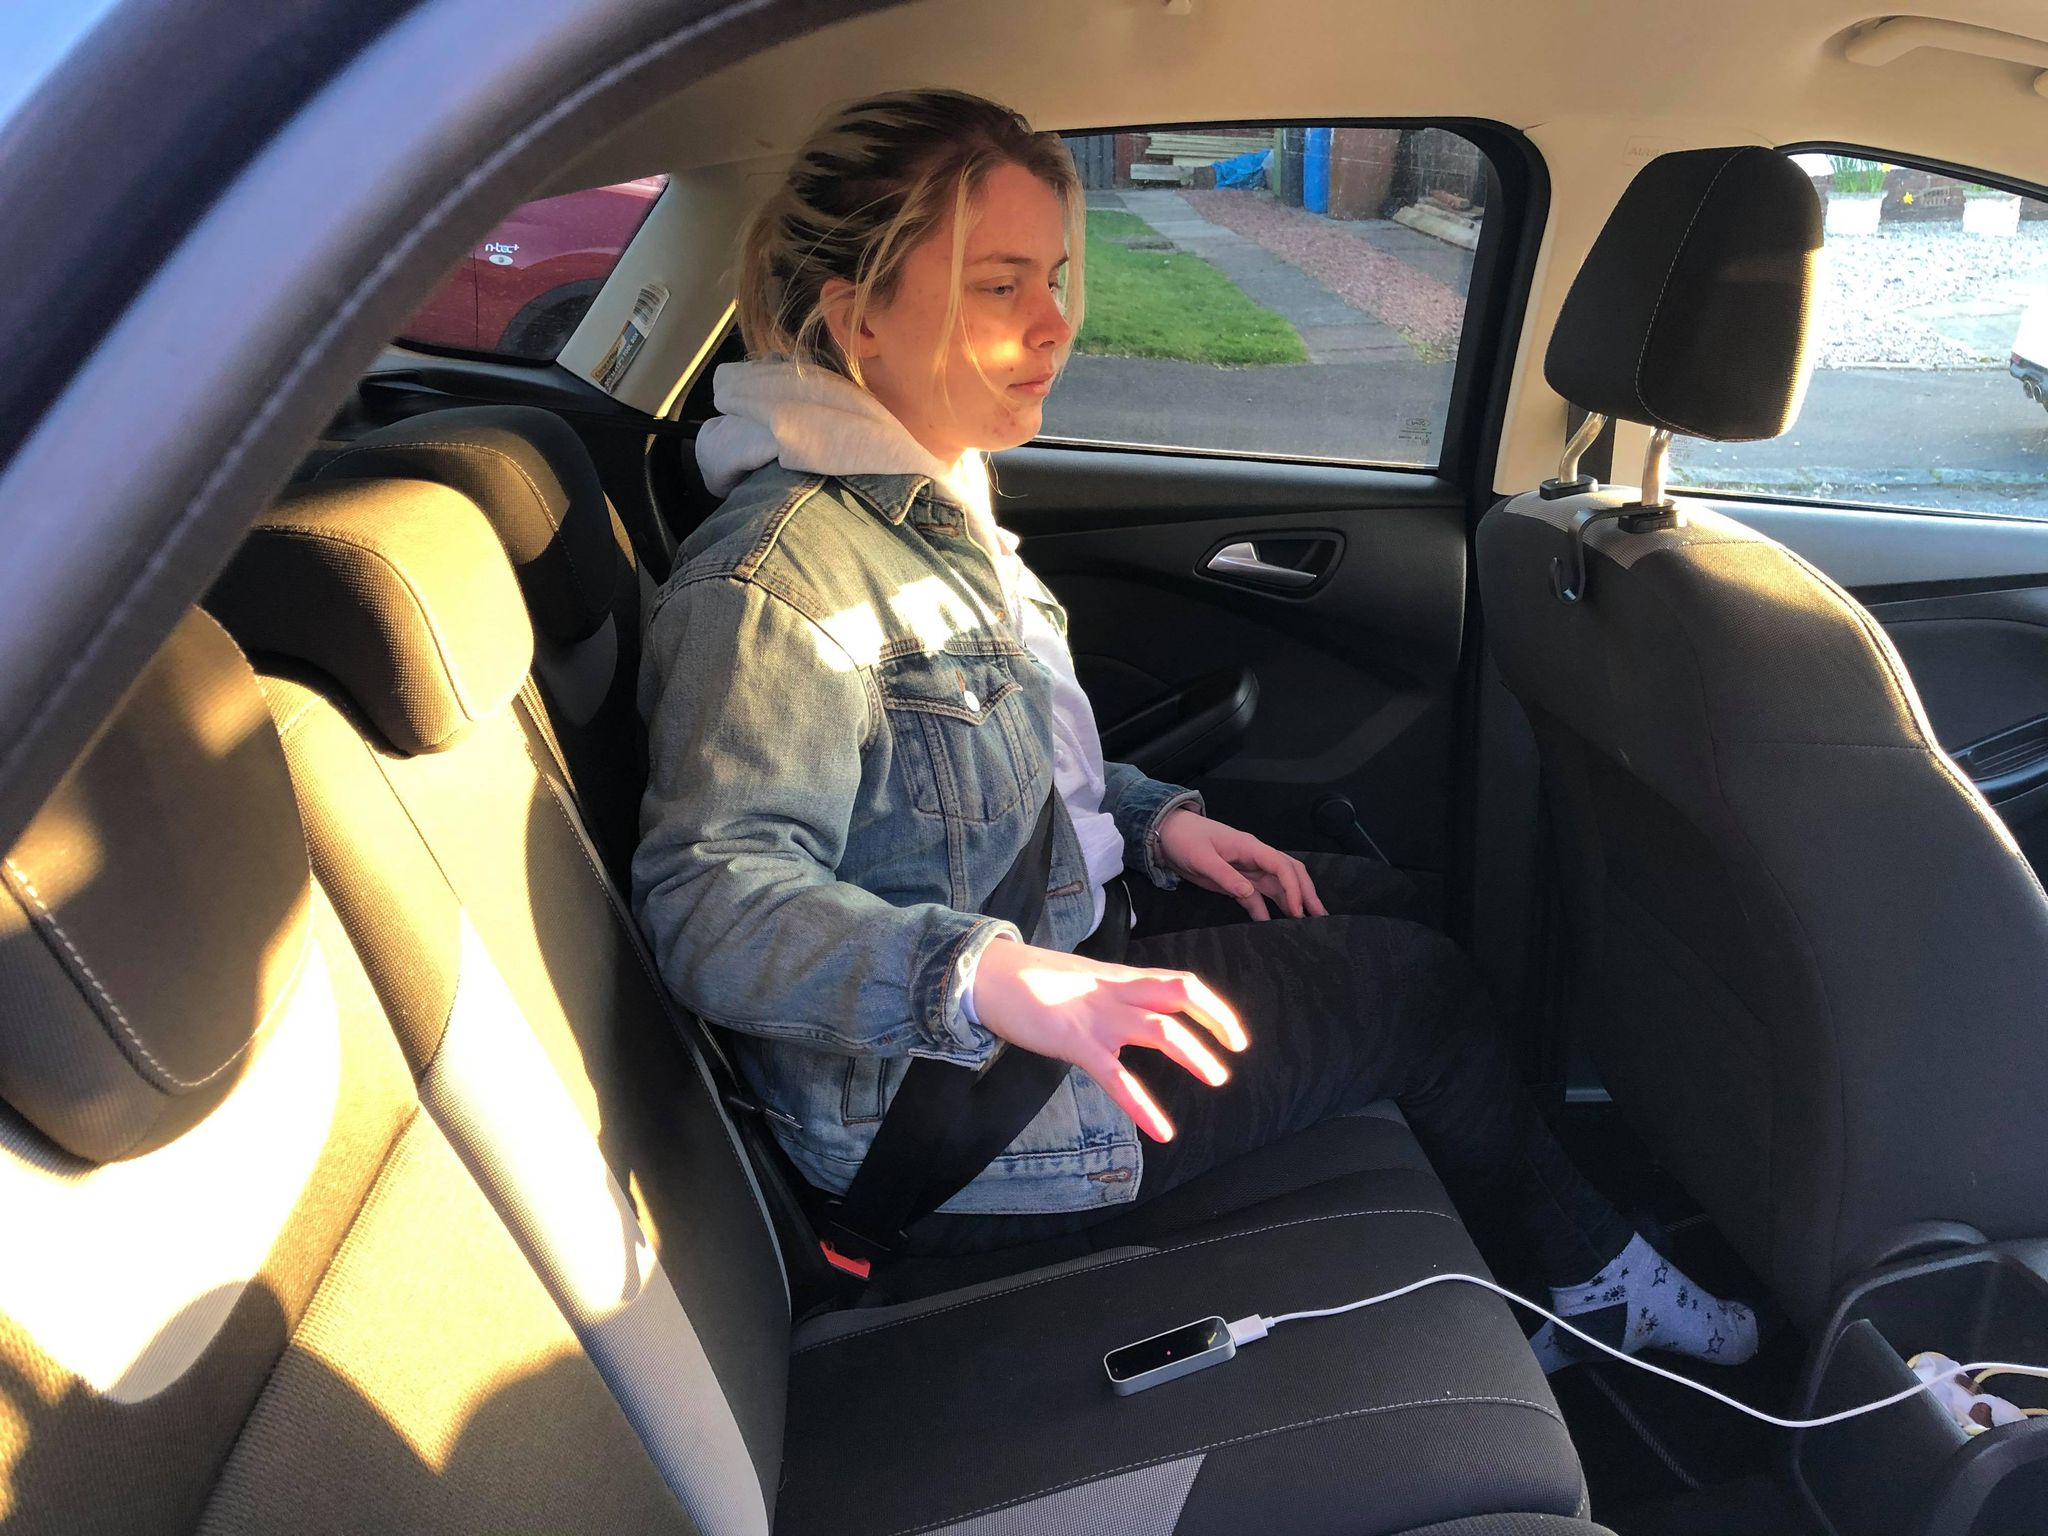
\includegraphics[scale = 0.08]{images/experimentSetUp2.jpg}
        \caption{Sensor to Side of Participant}
        \label{fig:setUp2}
    \end{subfigure}
    \caption{Experiment Set-Up}
    \label{fig:expSetUp}
\end{figure}

\section{Experiment}
The experiments took place in January 2021 and it took several days to complete. Before the experiment took place, all participants were asked to fill out a consent form which gave permission for their data to be used. The experiment was set up as described in the previous section each day that it took place. Participants were asked not to discuss any aspect of the experiment with anyone else until all participants had finished the experiment. This ensured that no one was advantaged and that the responses of participants were not influenced by another opinion. Each experiment took approximately an hour to complete which was much longer than anticipated. Participants were asked to go to the car and sit in whatever seat they were most comfortable. The evaluator sat in the front passengers seat and set the Leap Motion sensor up in front of the participant. 

The participant was then read the introduction and information sheet and were asked for their verbal consent. They were then given time to ask any questions they had regarding the experiment. Once the passenger was comfortable and had their seat belt on, the experiment started. Each participant was given the scenarios in a random order which had been previously created using an online random list generator. The evaluator then demonstrated the gesture that corresponded to a scenario as many times as the participant needed. They then performed the gesture themselves in front of the Leap Motion Sensor until they received the feedback that showed they had performed the gesture correctly. After all the scenarios had been completed once, the participant was then asked to perform them again but without a demonstration beforehand. This concluded Condition 1 and participants were asked to fill out a workload survey. Condition 2 followed the same structure as Condition 1 except that the sensor was then placed next to the participant. Once the participants had completed the scenarios twice, they were asked to fill out a workload survey for Condition 2 and then a general questionnaire. 

\section{NASA Task Load Index}
The NASA TLX was created as a tool to help measure the subjective workload of a user interacting with an interface. There are seven categories in which the participant must rate how they felt from low to high. These categories include mental demand, physical demand, time pressure, effort expended, performance level achieved, frustration experienced and annoyance experience.

The experiment was conducted under two conditions, the first being the sensor positioned in front and the second being the sensor placed to the side on the centre console. Under each condition, ten tasks were carried out and then repeated. On completion of tasks under the first condition, they were asked to fill out a NASA TLX survey and likewise, on completion of tasks under the second condition. These were kept together so that the workload for each condition could be compared for individual participants. Before filling out the NASA TLX surveys, each participant was asked to read the corresponding information sheet (Appendix \ref{section:TLXInfoSheet}).

\subsection{Results}
To analyse the TLX workload surveys, Excel was used. This was done by processing the raw data (Appendix \ref{section:TLXResults}) into tables. For example, there were tables for each condition which held each participant scores for that particular condition. Then a table of the average workload score for each category between the two conditions was created from these tables. 

Tables were created to compare a participant’s score for condition one and condition two. However, this was not seen to be particularly useful data, so it was not used any further. 

Following this, tables were created for each category comparing each participant’s score for condition one and two. This data was much more valuable as it showed a comparison between conditions and participants. 

Finally, a total workload table was created. The total workload was calculated by summing a participant’s score for each condition.

In total, there were 9 graphs created: one for average, one for total workload and 7 for each of the TLX categories. 

To gain insight into whether the results from the surveys were statistically significant a Paired T-test for Means was undertaken. This type of test is conducted when an experimenter wants to compare two values. In this case, the two values being compared were the scores for each condition. A result is said to be statistically significant if its P-value is less than 0.05.

Using this information, it was clear that the only two categories from the workload survey that were statistically significant were Performance Level Achieved and Time Pressure. 
 
Performance Level Achieved received a P-value of 0.037165187 as shown in figure \ref{fig:pLTable}. This suggests that participants found that they performed a lot better under one condition than the other. This is clearly shown in graph \ref{fig:pLGraph} where it was found that 6/8 participants felt they achieved better results under condition 2 and one participant felt they performed to the same level under both conditions. A reason they potentially thought they did better could be that they had grown used to performing the gestures and they felt more confident performing them. However, performing the gestures in the different positions did alter how the gestures were performed. The most likely reason for this score would be that they became more confident while participating in the experiment.
 
 \begin{figure}[!htb]
    \centering
    \begin{subfigure}[b]{0.45\textwidth}
        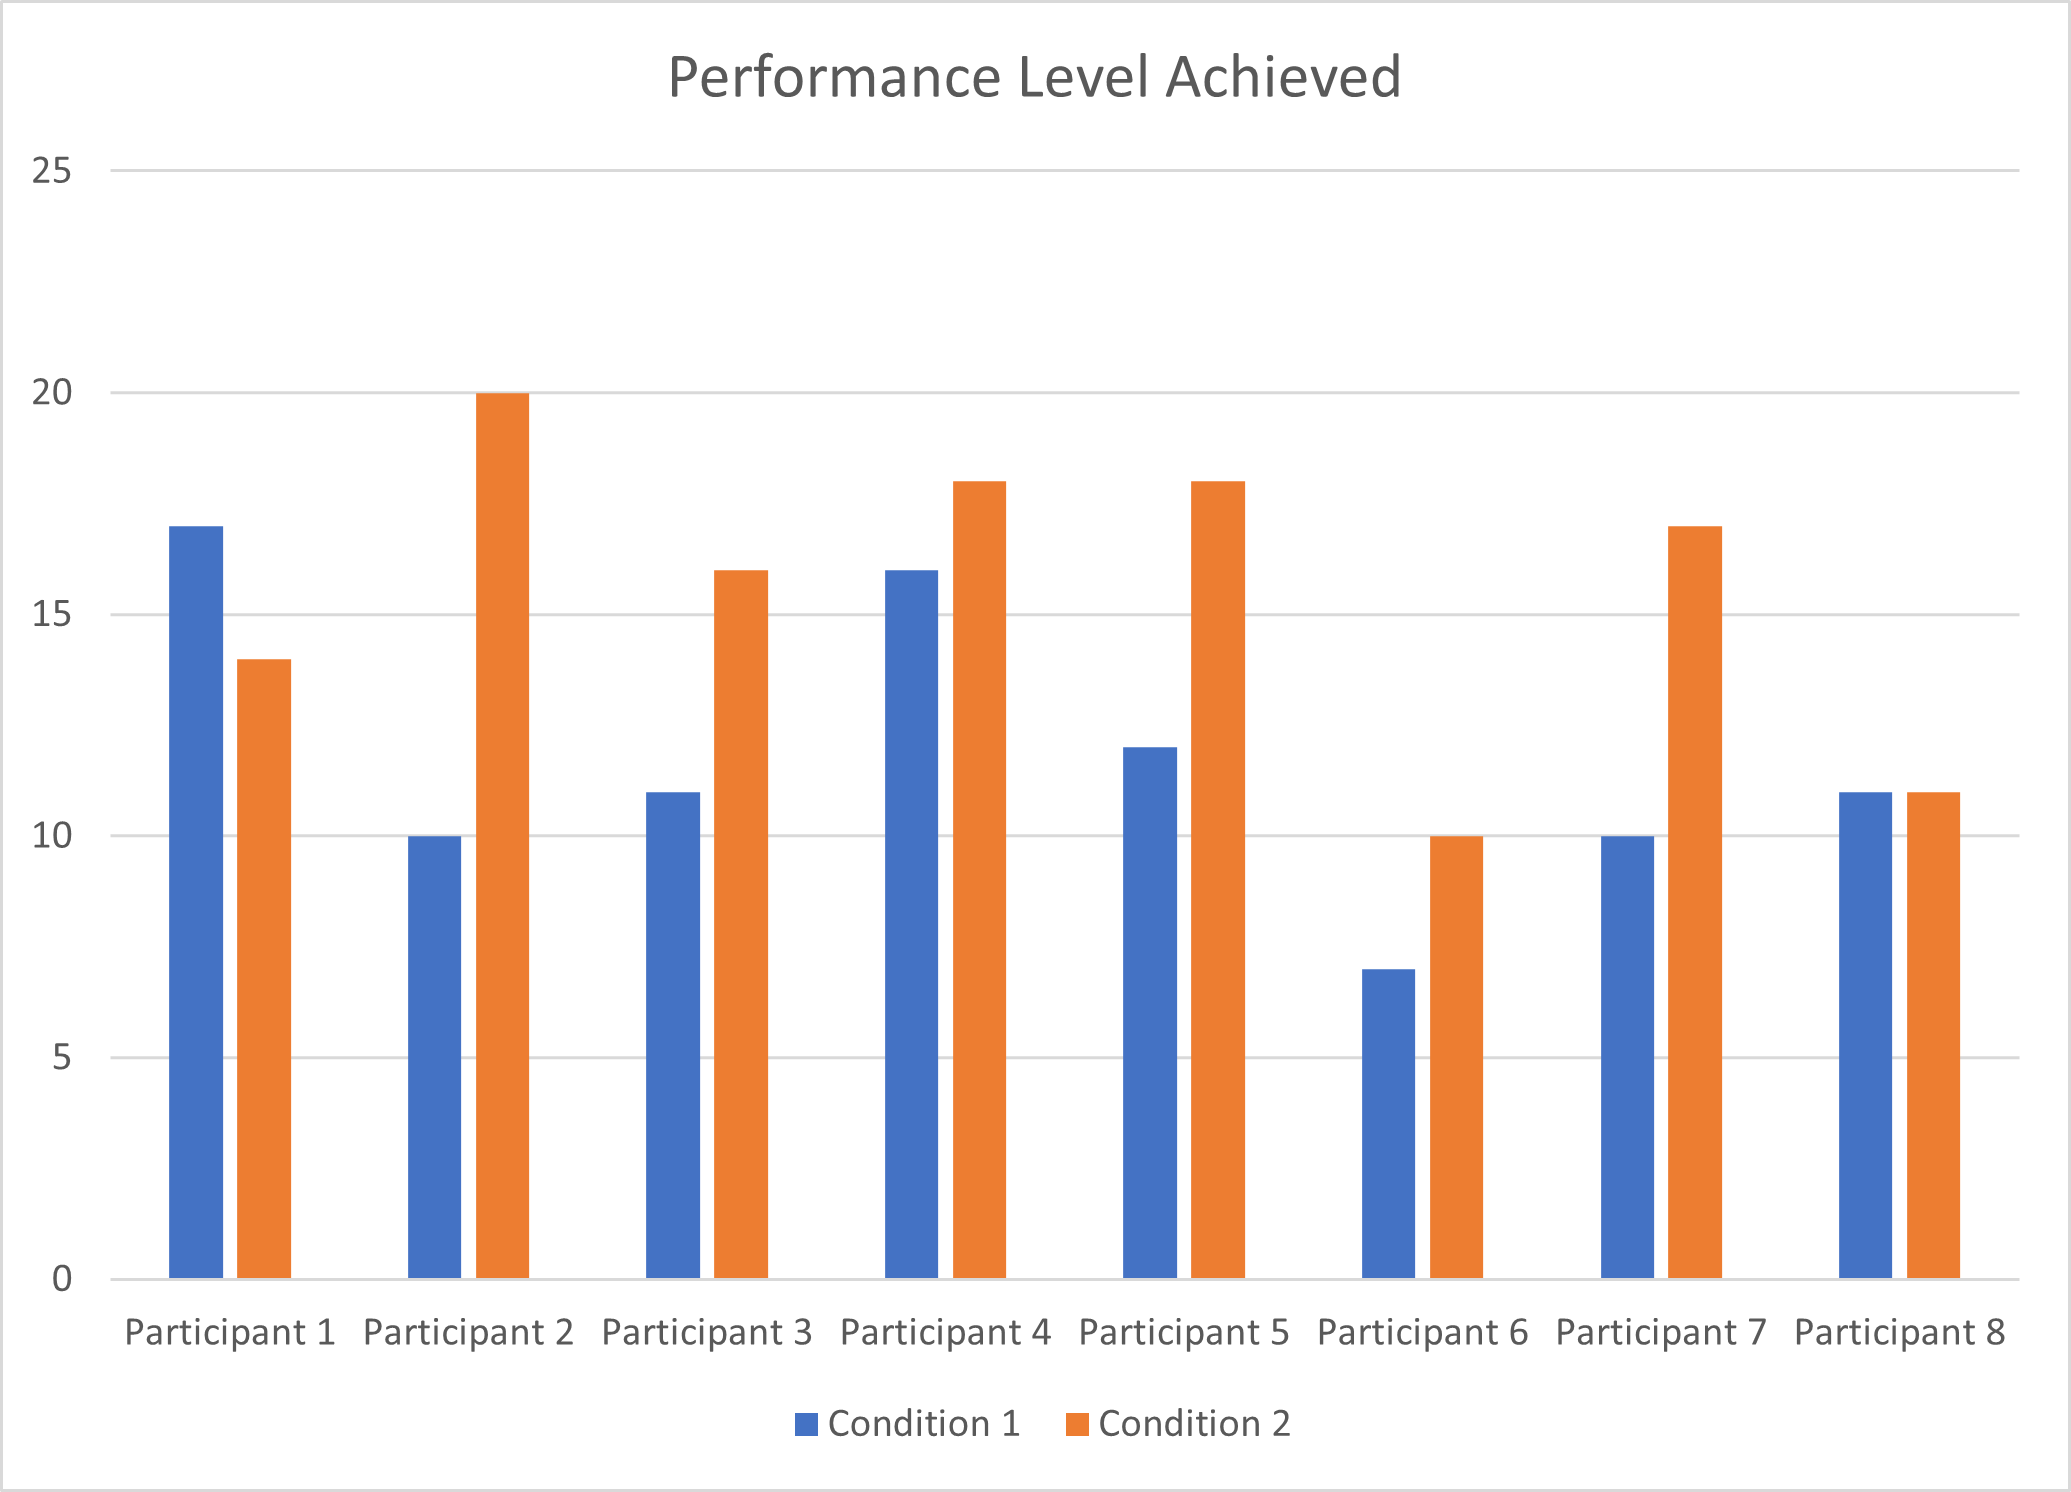
\includegraphics[scale = 0.4]{images/PerformanceLevelAchievedGraph.png}
        \caption{Performance Level Achieved Graph comparing both Condition 1 and 2}
        \label{fig:pLGraph}
    \end{subfigure}
    \begin{subfigure}[b]{0.45\textwidth}
        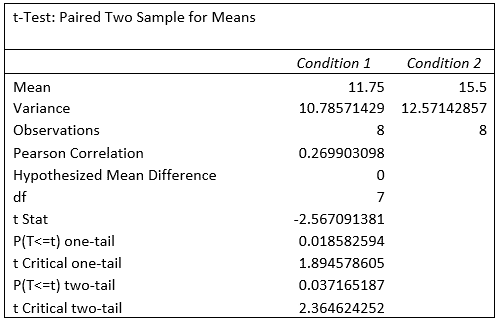
\includegraphics[scale = 0.55]{images/PerformanceLevelAchievedTable.png}
        \caption{Performance Level Achieved Table - Paired T-test}
        \label{fig:pLTable}
    \end{subfigure}
    \caption{Results of Performance Level Achieved Category from NASA TLX Workload Survey}
    \label{fig:PerformanceLevel}
    
\end{figure}

Time Pressure received a P-value of 0.035425164 which indicates that the participants felt like one condition had more pressure to complete on time than the other. This is surprising as there was no time constraint put on the participant to complete any of the gestures required. However, it could be that participants were putting the pressure on themselves and if they found a certain condition harder than the other then they may have felt extra pressure to get it done. From the bar chart that was created, it would appear as though participants found that there was more pressure put on them, time-wise, from condition 1. This could be partly due to the fact that it was the first condition that the participants faced and they didn’t know how to do the gestures properly yet.

The rest of the results from the other conditions were not considered to be statistically significant. However, this does not mean that their results are not important. Overall, the mental demand was found to be greater for Condition 1 over Condition 2 with it being voted more demanding by 4 participants compared to 2. The mean average was 9.5 for Condition 1 whereas Condition 2 only had a mean of 7.4. Physical demand had very mixed results with one participant saying that Condition 1 was 11 points more demanding than Condition 2.The rest of the results were a lot more balanced for Physical demand and this is shown from their means being only one apart.

On average, participants found the effort expended while performing both conditions to be very similar as the means are 7.25 for condition 1 and 7.125 for condition 2. The variance for condition 2 was much larger which suggests that even though the means were similar, participants either found condition 2 to be very low effort or very high effort.

Frustration experienced had a very large difference between the means for condition 1 and condition 2. This is also very similar for annoyance experienced. This could be due to them being a similar emotion. However, frustration experienced had a greater difference with condition 1 having a mean of 12.25 and condition 2 a mean of 8.875. This could suggest that although participants were frustrated while performing the gestures, it doesn't necessarily mean that they were annoyed by it. 

As previously mentioned, the total workload was taken to be the sum of the participants scores for each condition. This was a very important result to look at as it shows overall how 'hard' the experiment was. The graph and paired t-test is outlined in Figure \ref{fig:workload}. As can be seen from the graph, there are also very mixed results. The means show that they are fairly similar in terms of workload with condition 1 having a mean of 66.5 compared to condition 2 having a mean of 59. 

\begin{figure}[!htb]
    \centering
    \begin{subfigure}[b]{0.45\textwidth}
        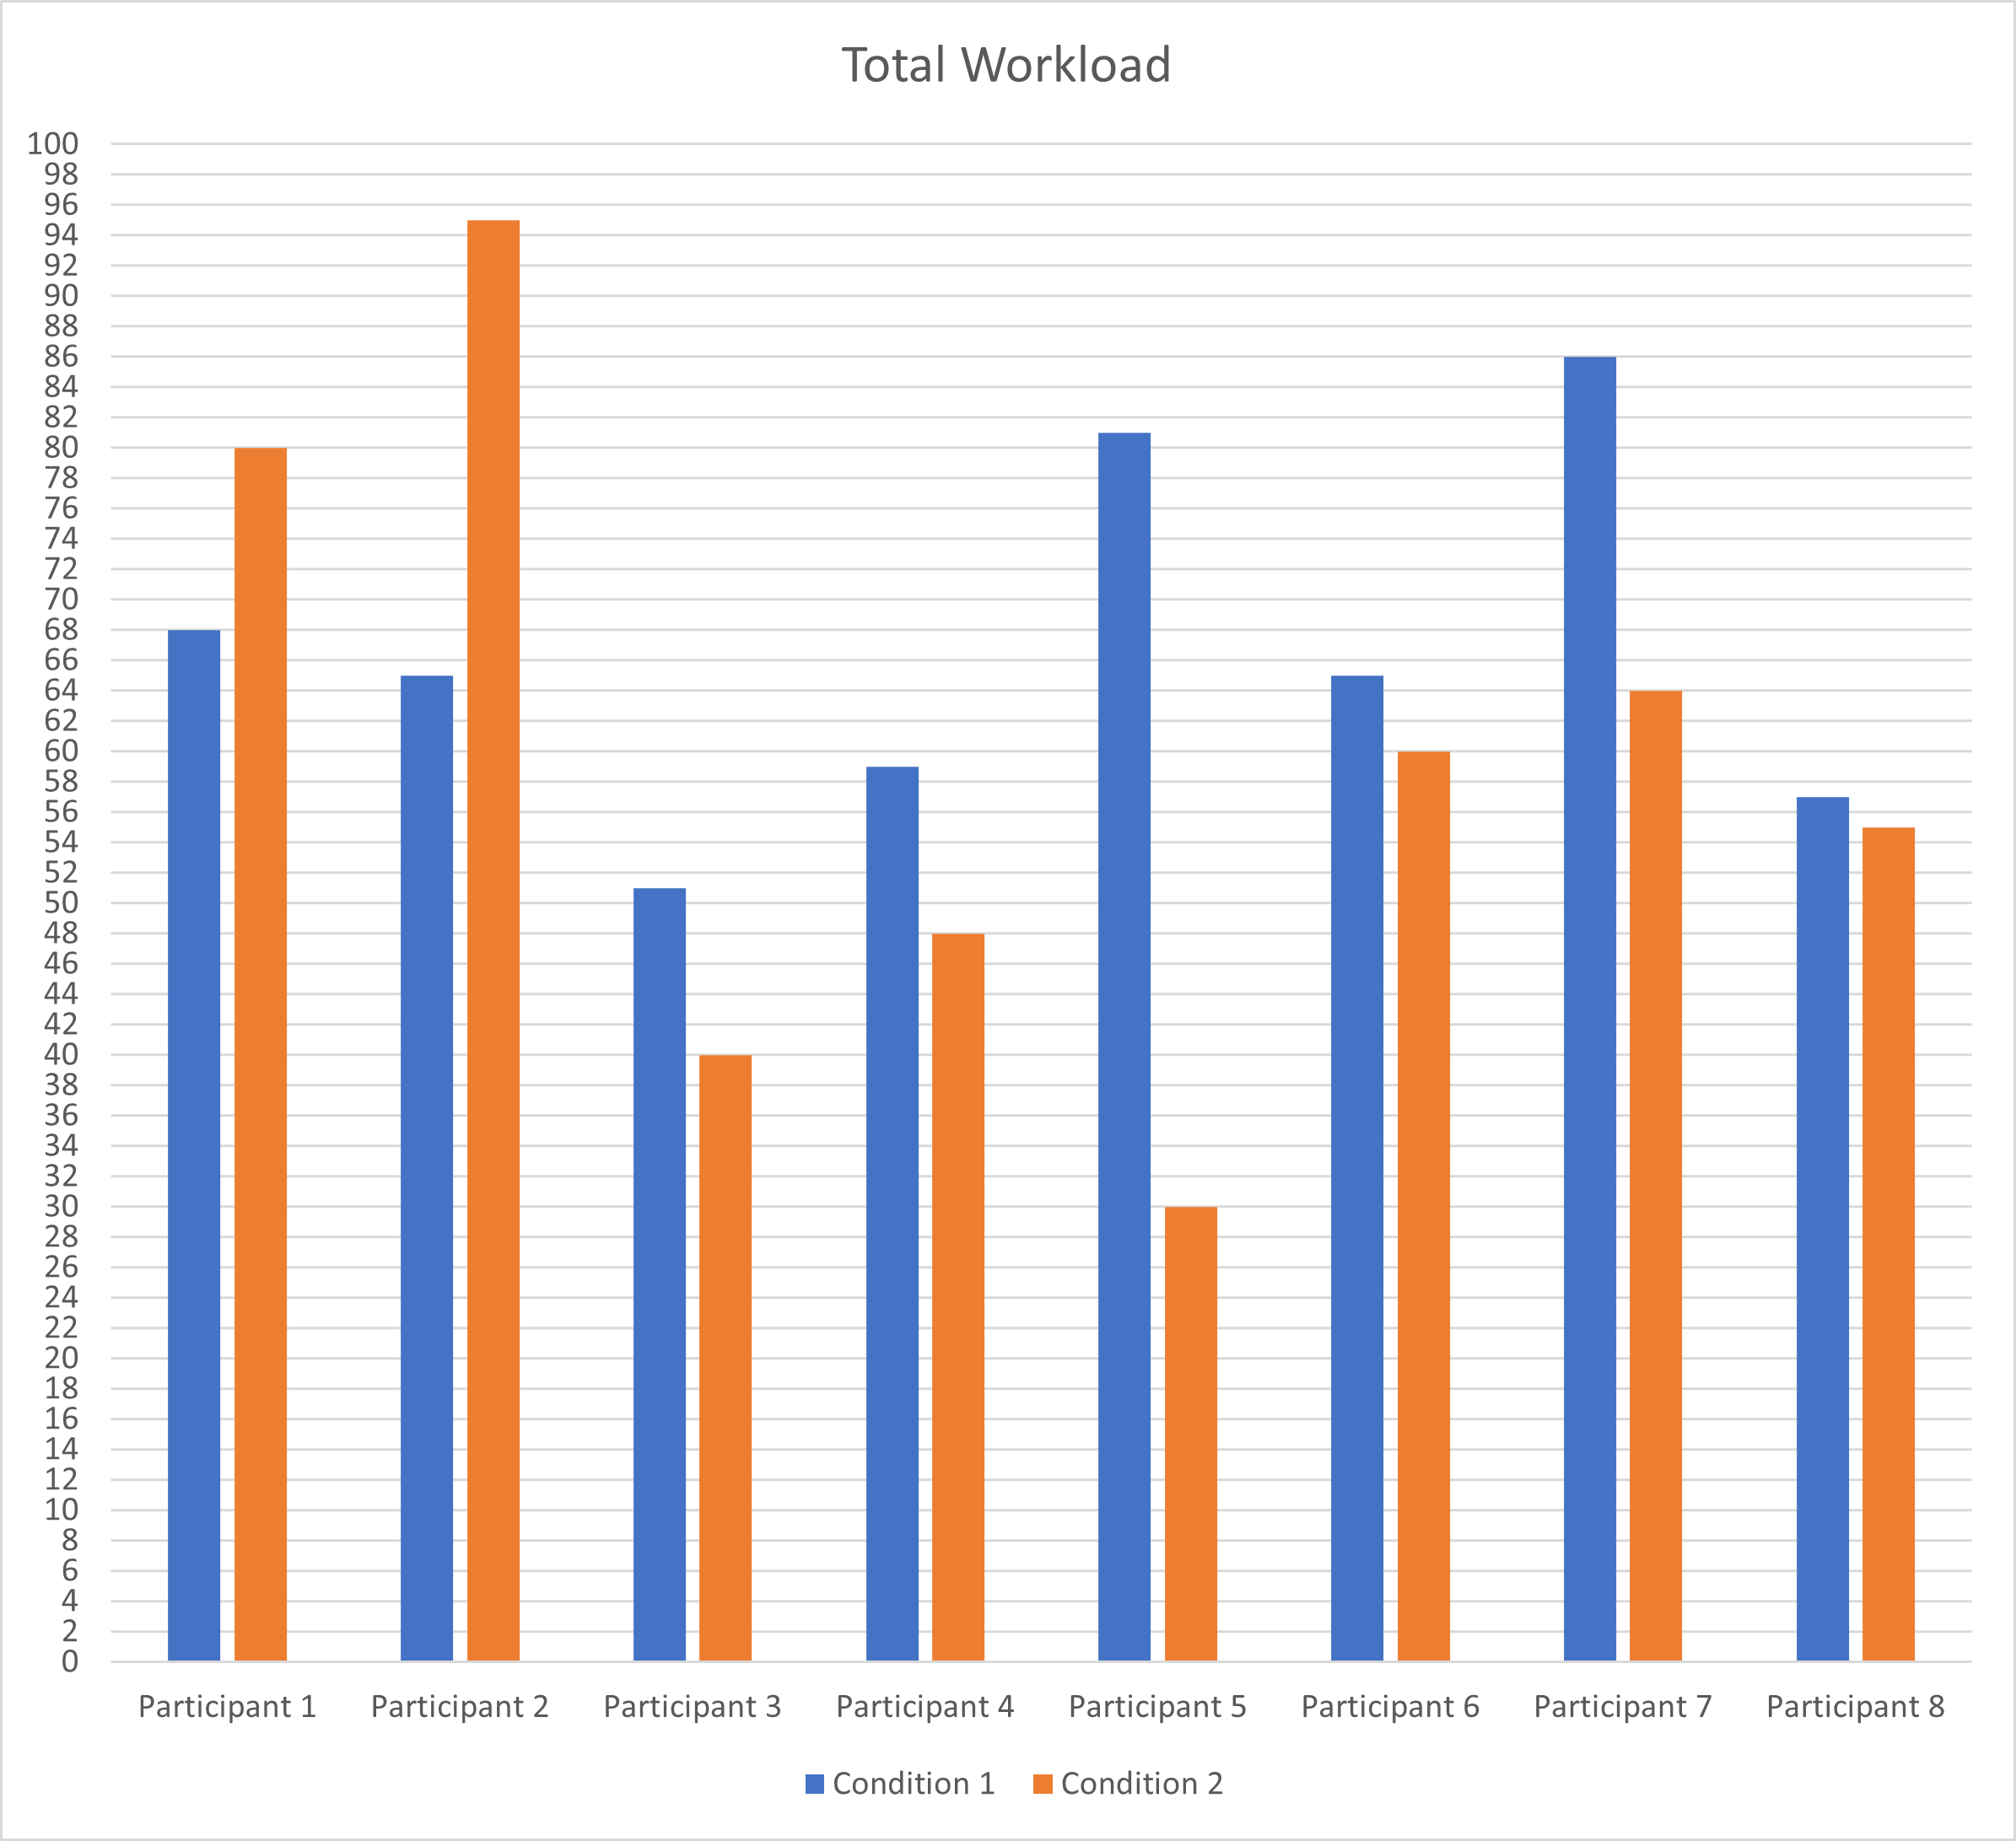
\includegraphics[scale = 0.5]{images/TotalWorkloadGraph.png}
        \caption{Total Workload Graph comparing both Condition 1 and 2}
        \label{fig:syn1}
    \end{subfigure}
    
    \begin{subfigure}[b]{0.45\textwidth}
        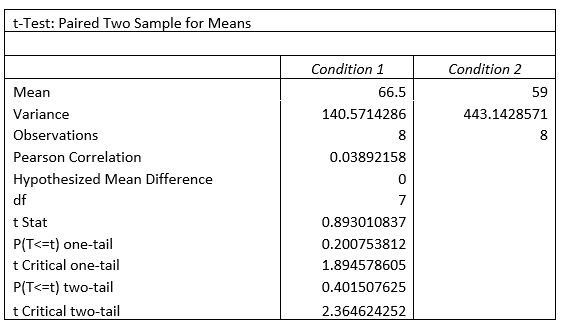
\includegraphics[scale = 0.6]{images/TotalWorkloadTable.png}
        \caption{Total Workload Table - Paired T-test}
        \label{fig:syn2}
    \end{subfigure}
    \caption{Results of Total Workload from NASA TLX Workload Survey}
    \label{fig:workload}
\end{figure}

\section{Surveys}
Originally a survey was created for the participants to complete after they had participated in the experiment. However, the questions ended up being vague and too open-ended. This resulted in responses that were not particularly meaningful or helpful and it was hard to gather conclusions from them. 
The survey was split into three sections: Feedback, Gestures, Position. Unfortunately, they had all been put on the same page which may have been overwhelming for the participant and it would have been easier for them to have been separated over three pages so there was less confusion between sections. 
For example, when asking the participant what they liked or disliked about feedback for a gesture, they would not specify if what they were saying was positive or negative. Furthermore, a lot of participants actually said what they liked or disliked about the gesture rather than the feedback. This was due to poorly worded and vague questions and lead to some questions being unable to be used in evaluating. 
To combat these issues, a follow-up survey was created and the questions can be seen in Appendix \ref{section:expSurvey}. This survey was sent out to participants a couple of weeks after participating in the experiment. There were a few concerns regarding their recollection of the gestures and/or feedback but they were encouraged to reach out if they needed any additional information or help with the survey. Fortunately, everyone was able to complete the follow-up without any problems. 
The follow-up survey was split into the same three sections as before, but also included an additional section which covered general questions regarding the experiment. Furthermore, the feedback section was not included, but instead, a usability section was added. After noticing the previous error with the sections, these sections were split over 4 pages so that there was no confusion for the participant.
The usability section in the second survey was based off of the 10 Usability Heuristics for User Interface Design by Jakob Neilsen. Some of these heuristics did not directly apply to the system that had been created so there were only 8 questions in total. However, some of the questions were split into two parts to ask for more detail as to why they chose an answer. 
There were 24 questions in the first survey and 57 questions in the second survey. There was an overlap between the questions as some in the second survey were very similar to ones in the first. This was due to needing clarification on some of the questions as they were previously not asked properly. 

\subsection{Results}
\subsubsection{Usability} 

All participants either agreed or strongly agreed that the feedback pages were consistent and easy to understand. They also agreed that the pages had just enough information and were not overly cluttered. This reinforces that it was a good idea to keep the design simple so that the users would understand it better. Furthermore, all participants also agreed that the symbols and animations used were easy to understand with further feedback explaining that there was a “clear change in visuals when gesture was done correctly” and that “most of them obviously corresponded to the gesture”. Only one person was ever unsure when they were doing the gesture correctly as they found that “sometimes the gestures were a tad confusing”. However, the rest of the participants felt as though they knew when the gesture was being performed correctly as they could see it from the screen registering their gesture by displaying feedback. 

All participants agreed that they would have benefitted from some form of error message letting them know if they were performing a gesture incorrectly. Some examples of the type of error messages were prompts, buzzers or sound. One comment in particular was very insightful and suggested that they could receive a pop-up that gives suggested actions close to the gesture that was being performed and the user could select which one they were attempting to perform. Another question that had been asked was if the participants would have liked the option to start over and only two participants said they would with one of them saying that they “possibly ‘over-did’ the gesture and would like to have started again”. This is a reasonable response to this as sometimes it could be hard for the participant to know when they should start again after continually performing a gesture incorrectly. On the other hand, some participants found it unnecessary  and had realised if their hand was kept away for long enough from the sensor then it would technically “reset” the gesture. 

Overall, these results suggest that the participants found the experiment usable.

\subsubsection{Feedback}
The participants all agreed that the feedback provided was appropriate for the experiment. However, they were given the option to select any other type of feedback that they thought would be appropriate and there was only one user who thought that the animations alone were enough. 6/8 participants thought that adding some audio would be useful. However, one participant did comment that any audio would perhaps disrupt any other audio in the car and could be annoying. Audio could be a feature that users are given the option to add in on top of the animations, but they don’t necessarily need it to use the system. 
Video and tactile feedback were also chosen by four people each as the participants had the ability to select more than one option. This shows that users would potentially like multiple feedback types at once or to be able to select their preferred method.
Words that were used to describe how people felt about these features included engaging, rewarding and interactive

\subsubsection{Gestures}
As previously mentioned, this section had to be revised as the questions in the first survey for the gestures were poorly worded and meaningful results were not able to be extracted from the majority of the answers. Since the follow-up survey was completed a couple of weeks after the experiment, the participants were given a video reminder of how each gesture was meant to be performed facing forward. After watching the video for a specified gesture and the corresponding control, they were asked in three separate questions what they liked, disliked, and if they were to replace the gesture with any other, what would they replace it with. This is represented in Table \ref{fig:gestureSurvey} which highlights the positive comments, the negative comments and any further suggestions. Each individual answer was not included as there were very similar answers written by different participants. These were grouped into answers such as "easy to understand" or the "gesture was representative of the action". Some participants may not have said this exactly but they either explained it in more detail or said something similar. Furthermore, participants were made aware that they did not need to fill out these questions if they didn't have an answer so some questions had fewer responses than others.

\begin{figure}[!htb]
    \centering
    \begin{subfigure}[b]{1\textwidth}
        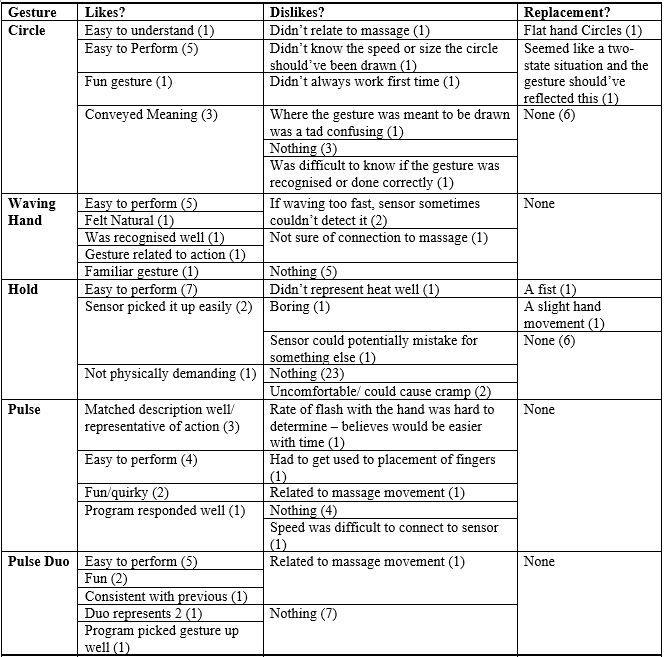
\includegraphics[width=15cm,height=9cm]{images/gestureSurvey1.png}
    \end{subfigure}
    \begin{subfigure}[b]{1\textwidth}
        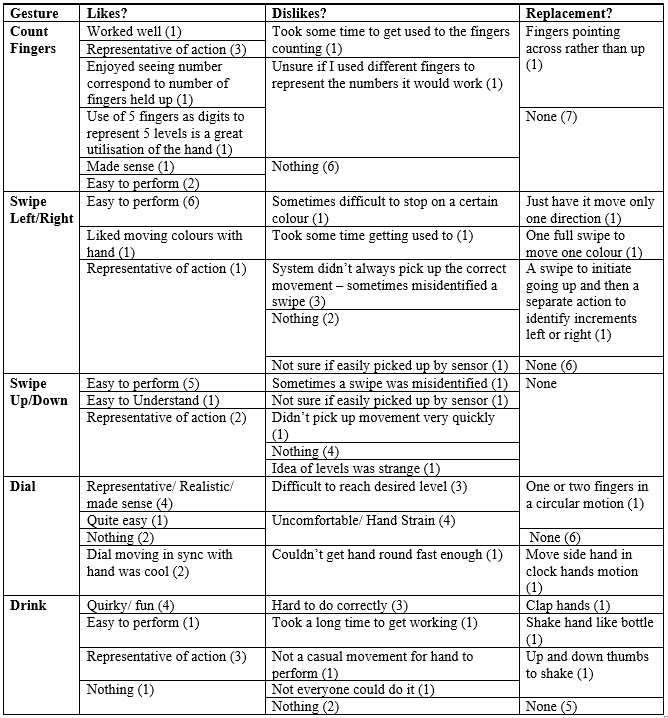
\includegraphics[width=15cm,height=10cm]{images/gestureSurvey2.png}
    \end{subfigure}
    \caption{Table showing the results from the gesture section of the follow-up survey}
    \label{fig:gestureSurvey}
\end{figure}

Assessing the gestures is a subjective task as the ease of performing them will vary from person to person. However, there were two gestures which clearly had more negative comments than positive. The dial gesture is one example of this as the comments were generally negative and the only significant positive comment related to it being representative of traditional action for adjusting temperature or volume (4 out of 6 participants said this). When looking at the negative comments, four participants complained of it being an awkward gesture to perform or that it caused hand strain. One participant commented that “The gesture was physically demanding and if you were expected to do this on a daily basis in worst case could result in RSI. The sensor did not pick up on the movements of my hand very well. I would turn the dial and the value would go up, however, when i went to make the second turn to increase it by more it then turned back down which caused a great deal of frustration.” which highlights that the usability of the dial gesture is not as high quality as some of the others.

On the other hand, there were quite a few of the gestures that received very positive feedback including "Waving Hand", "Pulse" \& "Pulse Duo", and "Counting Fingers".

\subsubsection{Position in Car}
This section was done in both surveys and this was due to the fact that, in the first survey, a lot of the answers were confusing. As the participants could pick where they sat, it was important to ask them if they felt comfortable performing the gestures in the seat they chose while gesturing to their side. 

Only 2 participants sat behind the passenger’s seat and both of them were right-handed and used their right hand to gesture. Both felt comfortable while performing the gestures and wouldn’t have changed where they sat.
However, out of the six participants who sat behind the driver’s seat only two of them used their left hand to gesture. This means that the remaining four participants had to stretch over their body to reach the sensor. Only two of these participants said that they found it uncomfortable. This could suggest that they maybe had shorter arms and it felt like more of a stretch or that the others did not mind stretching as much. Of the two participants who found it uncomfortable, only one of them said they would have preferred to sit in the other seat and the other person who would have preferred sitting in the other side had gestured with their left hand. This suggests it is just a preference thing as to where people would like to sit, rather than it having anything to do with how uncomfortable they are or if they are right or left handed. 

Following this, when gesturing forward 62.5\% of participants said that they did use a mixture of their right and left hand and everyone liked the flexibility of being able to use either hand even if they didn’t take advantage of it during the experiment. This result indicates that performing gestures facing forward may be preferable over gesturing to the side as users can use either hand without any discomfort. 

Finally, participants were asked which actions they currently perform in the backseat of the car and what gesture they thought best aligned with the action. As shown in Fig. \ref{fig:backseatGestures} there were four different actions that users said they did in the backseat. These show a variety of options that could be considered for backseat passengers to have control over using mid-air gestures in the future.

\begin{figure}[!htb]
    \centering
    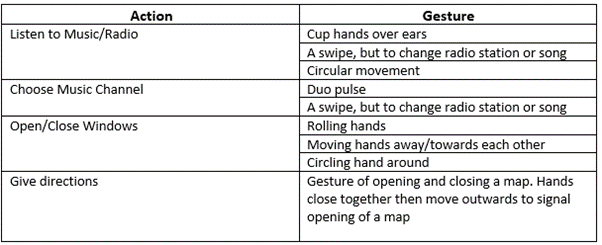
\includegraphics[scale = 0.8]{images/backseatGestures.png}
    \caption{Table of Actions and their Corresponding Gestures as suggested by survey participants}
    \label{fig:backseatGestures}
\end{figure}

\subsubsection{General}
Participants were initially asked what their favourite and least favourite graphics/ animations were. 
This was designed to elicit their preferred user interface whilst keeping the language non-technical. However, there were three participants who linked why they disliked an animation to how well they performed a gesture. This could be due to them not receiving the feedback as quickly as they would have liked when they struggled.

There were two favourite animations which were ‘Open Champagne Cooler’ and ‘Volume’. These both received 3 votes each. It was surprising that ‘Volume’ was a favourite whereas ‘Temperature’ received no votes as they were designed very similarly except ‘Temperature’ made more use of colour. ‘Volume’ and ‘Open Champagne Cooler’ had very contrasting designs. ‘Volume’ was very basic whereas ‘Open Champagne Cooler’ had spinning stars and a champagne bottle. This shows that people had a preference between very minimalistic designs and more creative designs. Participants both enjoyed the familiarity of the numbers increasing and decreasing on the screen to show the volume changing and the “visually rewarding” stars. 

The least favourite animations were ‘Ambient Lighting Colour’, ‘Hot Stone’ and ‘Massage Chair On/Off’ with 2 votes each. Some of the reasoning behind participants disliking these were that they were too simple or basic and not as rewarding. One participant said that the animation of rocks moving was not that “thrilling” and another said that the simplicity of the massage chair graphics was good but “not much more than that”. This suggests that users do like simple designs but also appreciate a design which is visually engaging. 

Participants were asked if they would use mid-air gesturing if it was a feature implemented in cars and all participants agreed they would with comments including it being “easier than voice activation” and “safer than asking the driver to make changes”. One participant even acknowledged that it is a feature that is already been implemented in the gaming industry and that seeing it become a part of everyday tasks would be interesting and novel. Overall, participants considered it an easier and safer option than manual switches or speech. Two participants did say that they would be uncomfortable performing the mid-air gestures if other people were around. However, one of the comments from the participants who said no claimed that it was fun and “something you would become used to”. This implies that they would potentially feel uncomfortable initially but would become more at ease as it becomes more mainstream. The other participant thought that it may seem strange to onlookers who may not fully understand why they are gesturing in a car. Some positive comments from participants included how cool and “futuristic” it could look to others and that they think it would be recognisable that they were performing gestures to control functions.  

\subsection{Conclusions Drawn}
In conclusion, it was found that the design of the experiment was usable and easy to understand. Participants understood when they were doing gestures correctly, but also believed they would have benefited from an error message whenever they were doing a gesture incorrectly. As previously mentioned, one participant did recommend that they could be given suggested gestures on the screen that are similar to what they were trying to do. This could be done by incorporating a yes or no feature with gestures and including a thumbs up and down to indicate this. This feature could make it easier for passengers who have difficulty performing certain gestures. Another important detail is that participants could see there being a benefit in having multiple feedback modalities such as audio, tactile or video. It was noted, however, that audio feedback could be a distraction over other audio playing in the car so it may not be the best option. 

It was discovered that the majority of participants were comfortable in either seat to perform the gestures. There were only a couple of participants who found sitting behind the driver uncomfortable when gesturing to their side. This could be due to them being right-handed and having to stretch across themselves to perform the gestures. This could suggest that having the sensor in the centre console may not be suitable for all passengers. Passengers appreciated the flexibility of being able to use either hand while gesturing forward which indicates that having the sensor facing forward may be the most suitable position. 

The participants had to perform 10 different gestures and were asked to give their opinions on them. It was found that gestures that required a little bit more precision such as dial or drink had more dissatisfied participants with some of them saying that they liked no aspect of these gestures. Conversely, there were many positive aspect that participants picked up on. They found that these gestures were highly representative of the action they were performing. 

Counting fingers received some of the least negative feedback with 6 people saying there was nothing they disliked about it.

Following this, participants were asked general questions about the experiment where it was discovered that the most popular animations were the ones for opening the champagne cooler and volume. The least favourite animations were the ones for ambient lighting, hot stone massage and turning the massage chair on and off. This was due to them being quite simple which was seen as a positive as well. It was decided that this meant that users like a minimalist design but they also like it to have more engaging and rewarding features like the spinning stars. 

Furthermore, all participants agreed that they would use mid-air gestures if they were implemented in their cars which is a promising result. This means that they all enjoyed performing the mid-air gestures and consider them to be a worthwhile feature to be implemented in cars that would make travelling safer.



\section{Issues}
\subsection{Covid-19 Impact}
Due to Covid-19, a few aspects of the experiment were unable to be completed as originally planned. For instance, the experiment should have taken place in a controlled environment within the university. This would have used a set-up that has been designed previously for participants to feel as though they are in a car. This allows for any random variables to be minimised. However, the experiment had to take place in the backseat of the most readily available car and the conditions were kept as controlled as reasonably possible. Unfortunately, there were some conditions that could not be controlled such as the lighting. Having to work around other people’s schedules meant that the experiments were being done at different times in the day and even on different days. The lighting in the car could affect how well the Leap Motion sensor detects gestures but by completing all the experiments during daylight would have aided this. 

Furthermore, there were not as many participants as would have been preferred. There were only 8 participants in total and they were all members of the same household and extended household. Fortunately, there was still able to be a varied participant set as there was a mixture of age and gender involved.

\subsection{Experiment}
The experiment took a lot longer than originally expected. Initially, the experiment was estimated to take up to 30 minutes per participant. However, it was more common for the participant to take an hour to complete the experiment. Including the questionnaire, it took most participants over an hour. This caused several problems with how the experiment progressed as the laptop being used frequently ran out of charge, therefore extending the length of time it took to complete the whole experiment.

Another issue that was identified post experiment was that, although the order in which the participant completed each scenario was randomised, the position in which the sensor started was not. This could cause users to get used to performing the gestures facing forwards and then be better at performing them while the sensor is at their side. This could unknowingly cause them to find performing the gestures to the side easier which could have skewed the data.


\section{Discussion}
In order to test if the gestures worked effectively in the backseat of a car, an experiment was conducted with 8 participants. This required them to perform a series of gestures and report on their perceived workload of them. This provided insight as to how difficult a user found a certain condition and overall, it was found that condition 1 and condition 2 had roughly the same workload. However, it was found that people felt while performing gestures in front of themselves, there was a greater time pressure perceived. Furthermore, participants found that they performed better performing gestures to their side than in front of themselves. 

The rest of the conditions were found to not be statistically significant and the overall workload varied from participant to participant. However, participants were more split on condition 2 as it received a wide range of results. Overall, condition 2 was found to have a lower workload than condition 1.

The results from the TLX surveys suggest that it would be most practical to have two sensors in the car so that users could choose which one they wanted to use. This would allow users to not have to be tied to one sensor, especially if they are uncomfortable with that position. 

Following the two TLX surveys, the participants were required to complete an online survey. The results from this survey were combined with another survey that was completed at a later date. Combined, it was discovered that there were several gestures that participants did not like. This included opening the champagne cooler and dial. Some people also disliked the swiping motion. Numerous comments highlighted that participants were frequently unsure if the sensor was detecting their hand properly. 

Participants found that the dial gesture was uncomfortable and caused their hand to strain and they also found it difficult to reach their desired level i.e. temperature or volume. Two participants could not think of anything they liked about this gesture and the main positive comments were that it represented the control well. This shows that the dial gesture needs a lot of improvement as participants did not enjoy the gesture. Another gesture that wasn't liked was the drinking gesture. Although novel, participants found it hard to do correctly and would potentially rather do a different gesture such as a gesture that looks like you are shaking a bottle.

\section{Further Development}
In order to address some key issues that arose from the experiment, one of the gestures from the gesture set was revised. As previously discussed, the dial and drink gesture received a lot of negative feedback from participants so it was decided that one of these gestures would be refined. 

The dial gesture was chosen as two of the participants couldn't think of any positive feedback for them and the majority of participants couldn't think of a gesture that would replace it. One way to refine this gesture was to introduce segmentation. Segmentation is used to help determine when a user is wanting to start performing a gesture. To aid with segmentation, a clutch can be used. A clutch is an action which means that the gesture being performed has become active. 

The dial gesture required a user to have an open palm and pretend to be turning a dial. To distinguish between a user performing the dial motion and accidentally moving their hand in the wrong direction, the user must close their hand into a fist when they are not going to perform the gesture. Furthermore, the threshold for difference in angles was increased, so if a user had a shakier hand or the road was bumpy, there would be less chance of any errors occurring. 

In order to evaluate if this gesture was more appropriate than the previous one, a small experiment was conducted. This consisted of four participants trialling the new gesture. This experiment was conducted similarly to the previous one but, due to time constraints, the gestures were only performed facing forwards. The participants were asked if they remembered the previous gesture and if they had any problems with it. They were then shown how to perform the improved dial gesture and asked to adjust the temperature. Following this, the participants were asked a series of questions in order to understand what they liked and disliked about the improved gesture. All of their responses were spoken, so it made most sense to record their answers and then create a table with what was said.

\begin{figure}[!htb]
    \centering
    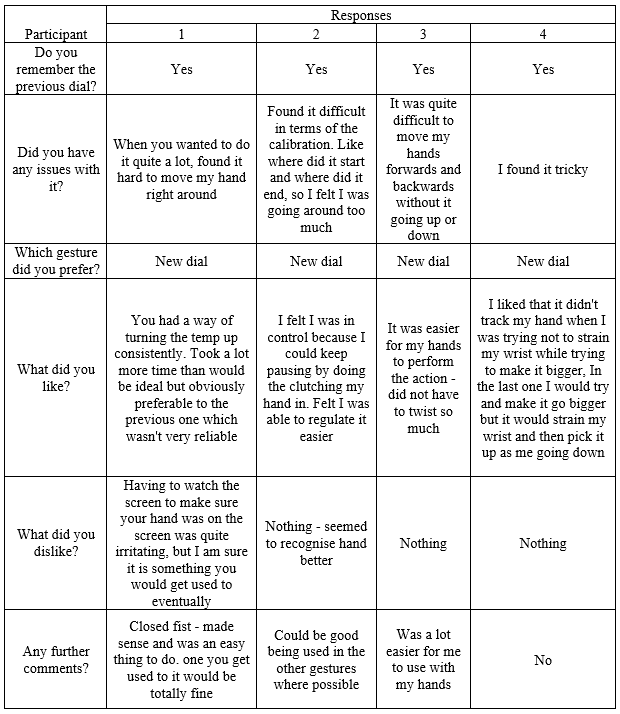
\includegraphics[scale = 0.8]{images/furtherGesture.png}
    \caption{Table of Results from Revised Dial Gesture}
    \label{fig:revisedGesture}
\end{figure}

The results from the experiment are shown in Figure \ref{fig:revisedGesture}. All of the participants preferred the new dial gesture as it was found to be easier and allowed them to have more control over the movement due to the "clutch" action. One participant said that it did take a bit longer than would be ideal and that it was inconvenient having to ensure your hand was always in the exact correct place. Furthermore, all of the participants found the previous gesture quite difficult. 

These results give promise that, if some gestures were previously disliked, by considering different options and adjusting them slightly, they can become easier to use and control.

%==================================================================================================================================
\chapter{Conclusion}    
\section{Summary}

Cars are a ubiquitous presence on our streets and in the lives of a very significant percentage of the world’s population. Their desirability ensures they are constantly developing and evolving. With advances in technologies happening in society at a faster pace than ever before, car makers are keen to fully exploit them to enhance the efficiency, reliability and safety of their vehicles. Additionally, passenger comfort has become an increasingly important consideration for car buyers with leading car brands competing to provide the best, and most luxurious, passenger experience, often facilitated by the latest technologies. This experience can include, among many features, mood lighting, massage chairs and entertainment systems. Enhancing the experience further can be the ease with which the features can be controlled. 

While there have been previous studies on using mid-air interactions within cars their main focus was on the drivers and the safety of the driving experience. This project focused on the use of mid-air interactions to control features inside a car from the backseat.

The project’s aim encompassed the following three questions:

\begin{itemize}
\item Which gestures do backseat passengers associate with actions they can do in the backseat of a car?
\item Which gestures can be implemented using the Leap Motion sensor?
\item How well are the gestures performed while sitting in the backseat of a car?
\end{itemize}

In order to address these questions, research was carried out into the different controls in the back of a car. These controls were based on Land Rover’s ‘luxury’ features which include massage chairs, ambient lighting and a champagne cooler. More basic features were also considered to ensure there was a wide range of controls that could be studied. 

In order to gain a better understanding into what potential end users thought would be appropriate gestures, two gesture elicitation surveys were completed. Gesture elicitation surveys aim to obtain a set of gestures and, in this case, it was to identify potential gestures that could be performed in the backseat of a car. Once this was completed, a gesture set could be created followed by the wireframes for the user interface. 

With the aim of developing a suitable experiment, research had to be carried out on the Leap Motion in order to learn whether it could correctly recognise the gestures in the gesture set. After thorough research and practice, ten experiments were created. This involved incorporating the Leap Motion with PyGame. PyGame was used to create the Graphical User Interfaces (GUI) so that the participants in the experiment could receive meaningful feedback on the gestures they were performing. 

The experiments, completed by eight participants, were conducted in the backseat of a car with the Leap Motion sensor positioned in an appropriate location.  Each experiment started with the sensor facing the participant and then it was moved to be beside them on the centre seat. The experiment involved the participants performing the gestures and completing two workload surveys and a questionnaire. Workload surveys are completed in order to determine the level of difficulty experienced by participants.

The results made it clear that there was significant potential for implementing mid-air gestures in the backseats of cars. However, a considerable amount of work will need to be done in order for this to be achievable. Participants were keen on the concept but were not always able to perform each gesture to as high a standard as they would have liked. This suggests that the gestures could be improved on. Furthermore, the feedback given was at a basic level to ensure the participants understood clearly if they were performing the gestures correctly. Only a graphical user interface was implemented, and this could be developed to include different feedback modalities such as audio or tactile to improve the user experience. 

Finally, if the development of mid-air gestures for passengers in cars is continued, a wider range of controls should be considered along with the different types of cars that they could be used in. Instead of only focusing on luxury brands, they could broaden the market and aim this technology at family cars. There are many opportunities for mid-air gestures to be incorporated in cars and it need not be limited to a certain type of car or set of gestures.

\section{Future Work}
Following a thorough evaluation of the experiment it became clear that there are numerous avenues for the future development of mid-air gestures for passengers in cars. 

\subsubsection{Environment}
This study was conducted in a controlled environment while the car was stationary. It is quite possible that passengers would perform the gestures differently if the car was moving. A reasonable next step could be having them test the effectiveness of gestures while the car was in motion. Of course, the experiment would still have to be controlled to a degree as there could be many random variables which could make all the experiments differ.

\subsubsection{Car Model}
The set up for the experiment was not as realistic as it could have been. The vehicle used was very different to a Land Rover and it could be assumed that, by using a vehicle closer in layout to the Land Rover, passengers would produce a more realistic result as to how the gestures would be performed. As such, further studies could be done in different car brands and models to compare the workload between cars. 

\subsubsection{User Interface}
Another important aspect to note is that a laptop was used to give feedback during the experiments. This differs from the luxury cars within which tablets are built into the backseats. By transferring the software to a tablet and attaching it to the backseat of a car, a more realistic experiment could be undertaken as the feedback would be provided in the most appropriate position. 

However, before any of these further studies can be conducted, it would be advisable to improve upon the gestures which have been created and make them more user friendly. Participants gave negative feedback about some of the gestures and, while also recognising significant positive feedback, it is important that any issues are addressed. Additionally, it would be worthwhile to improve the user interfaces and potentially make them more interactive by including audio or tactile feedback.

%==================================================================================================================================
%
% 
%==================================================================================================================================
%  APPENDICES  

\begin{appendices}

\chapter{Gesture Elicitation Survey}

\section{Participant Consent Form for the Gesture Elicitation Survey}
\label{section:ConsentGE}
The aim of this experiment is to learn about what gestures people will associate with different actions in a car if there was a sensor in the centre console of the back seat.

The survey will take roughly 30 minutes to complete.

Firstly, the format of the survey will be explained, and you will be asked to position your camera so that your hand is visible.You will then be asked a series of questions asking you to do some gestures that you deem appropriate to the action you will be asked about.  

Your gestures will be recorded over zoom to be reviewed later. All results will be kept private. However, no personal data will be stored and if you wish to drop out then all data recorded will be discarded. 

\begin{tabbing}
If you \=have any further questions about the survey, please contact:\\
\> Catriona Murphy\\

\>School of Computing Science\\

\>2312695m@student.gla.ac.uk\\

\end{tabbing}


I have read this information sheet, and agree to voluntarily take part in this experiment.

\textbf{Name:}\\
\textbf{Email:}\\
\textbf{Date:}\\

\emph{This study adheres to the BPS ethical guidelines, and has been approved by the DCS ethics committee of The University of Glasgow.. Whilst you are free to discuss your participation in this study with the experimenter, if you would like to speak to someone not involved in the study, you may contact the chair of the DCS Ethics Committee: Prof Stephen Brewster}


\section{Information Sheet for Gesture Elicitation Survey}
\label{section:inforSheetGE}
The aim of this experiment is to learn about what gestures people will associate with different actions in a car if there was a sensor in the centre console of the back seat.

The survey will take roughly 30 minutes to complete.

Firstly, the format of the survey will be explained, and you will be asked to position your camera so that your hand is visible.You will then be asked a series of questions asking you to do some gestures that you deem appropriate to the action you will be asked about.  

Your gestures will be recorded over zoom to be reviewed later. All results will be kept private. However, no personal data will be stored and if you wish to drop out then all data recorded will be discarded. 

\begin{tabbing}
If you \=have any further questions about the survey, please contact:\\
\> Catriona Murphy\\

\>School of Computing Science\\

\>2312695m@student.gla.ac.uk\\

\end{tabbing}

\emph{This study adheres to the BPS ethical guidelines, and has been approved by the DCS ethics committee of The University of Glasgow.. Whilst you are free to discuss your participation in this study with the experimenter, if you would like to speak to someone not involved in the study, you may contact the chair of the DCS Ethics Committee: Prof Stephen Brewster}


\section{Introduction Script For Gesture Elicitation Survey}
\label{section:introScriptGE}
The general aim of this experiment is to learn about what gestures people will associate with different actions in a car if there was a sensor in the centre console of the back seat. We require your participation so that we can see what gestures passengers would use in different scenarios while being driven about.

The experiment will require each you to sit in the back seat of your car, if you have one, or a chair in your house. For a more realistic participation, we ask that, if you do have access to a car, that you use this.

You will be asked 10 questions. These questions will ask you how you would do something using a mid-air gesture i.e. not using any buttons or dials.

I will observe what gestures you do and if you have any questions, you can ask at anytime during the survey.

It doesn’t matter what gestures you use as the aim of the survey is to gather as many different gestures as possible from participants. 

This survey will be done over Zoom and it will be recorded. If, at any time, you wish to withdraw from the experiment, just let me know. 

Do you agree to taking part in this survey?\\Do you have any questions before we start?

\section{Debrief Script for Gesture Elicitation Survey}
\label{section:debriefScriptGE}
The main aim of the survey was to learn about what gestures people associate with different actions in a car. However, I was also looking to see if you repeated any gestures for more than one action. This would imply that some actions may not be able to bedone using mid-air gesture interaction if it’s too similar to another action.\\
Do you have any comments or questions about the survey? If you have any further questions, then you have my contact details. Thank you for your help.

\section{Gesture Elicitation Survey Questions}
\label{section:GESurveyQ}

1. How would you change the temperature of the air conditioning? Think about turning the temperature up and down.\\
2. How would you recline your chair?
\begin{itemize}
    \item Think angle of the chair
    \item There is also a leg rest. How would you pull this out?
    \item Lumbar support -move to the top or bottom of the chair
    \item Need to pull it out and push back in?
    \item The headrest can be moved forwards, backward, up, and down. How would you indicate this?
    \item How would you inflate the side bolsters? And deflate?
\end{itemize}
3. How would you turn the volume up for the music?\\
4.How would u open the windows? And close?\\
5.How would you turn the massage chairs on?\\
6.There are 5 different formats. How would u set it to each format:
\begin{itemize}
    \item Wave
    \item Pulse
    \item Pulse Duo
    \item Combination
    \item Hot Stone
\end{itemize}
7.There are 5 intensity levels -how would you switch between each one?\\
8.How would you change the colour of the ambient lighting in the car?
\begin{itemize}
    \item There are 4 different brightness levels. How would you switch between each one?
\end{itemize}
9.How would you mute all audio in the car?\\
10.How would you open the champagne cooler? The door slides up and down in between the two back seats.

\section{Gesture Elicitation Processed Data}
\label{section:analysisGE}
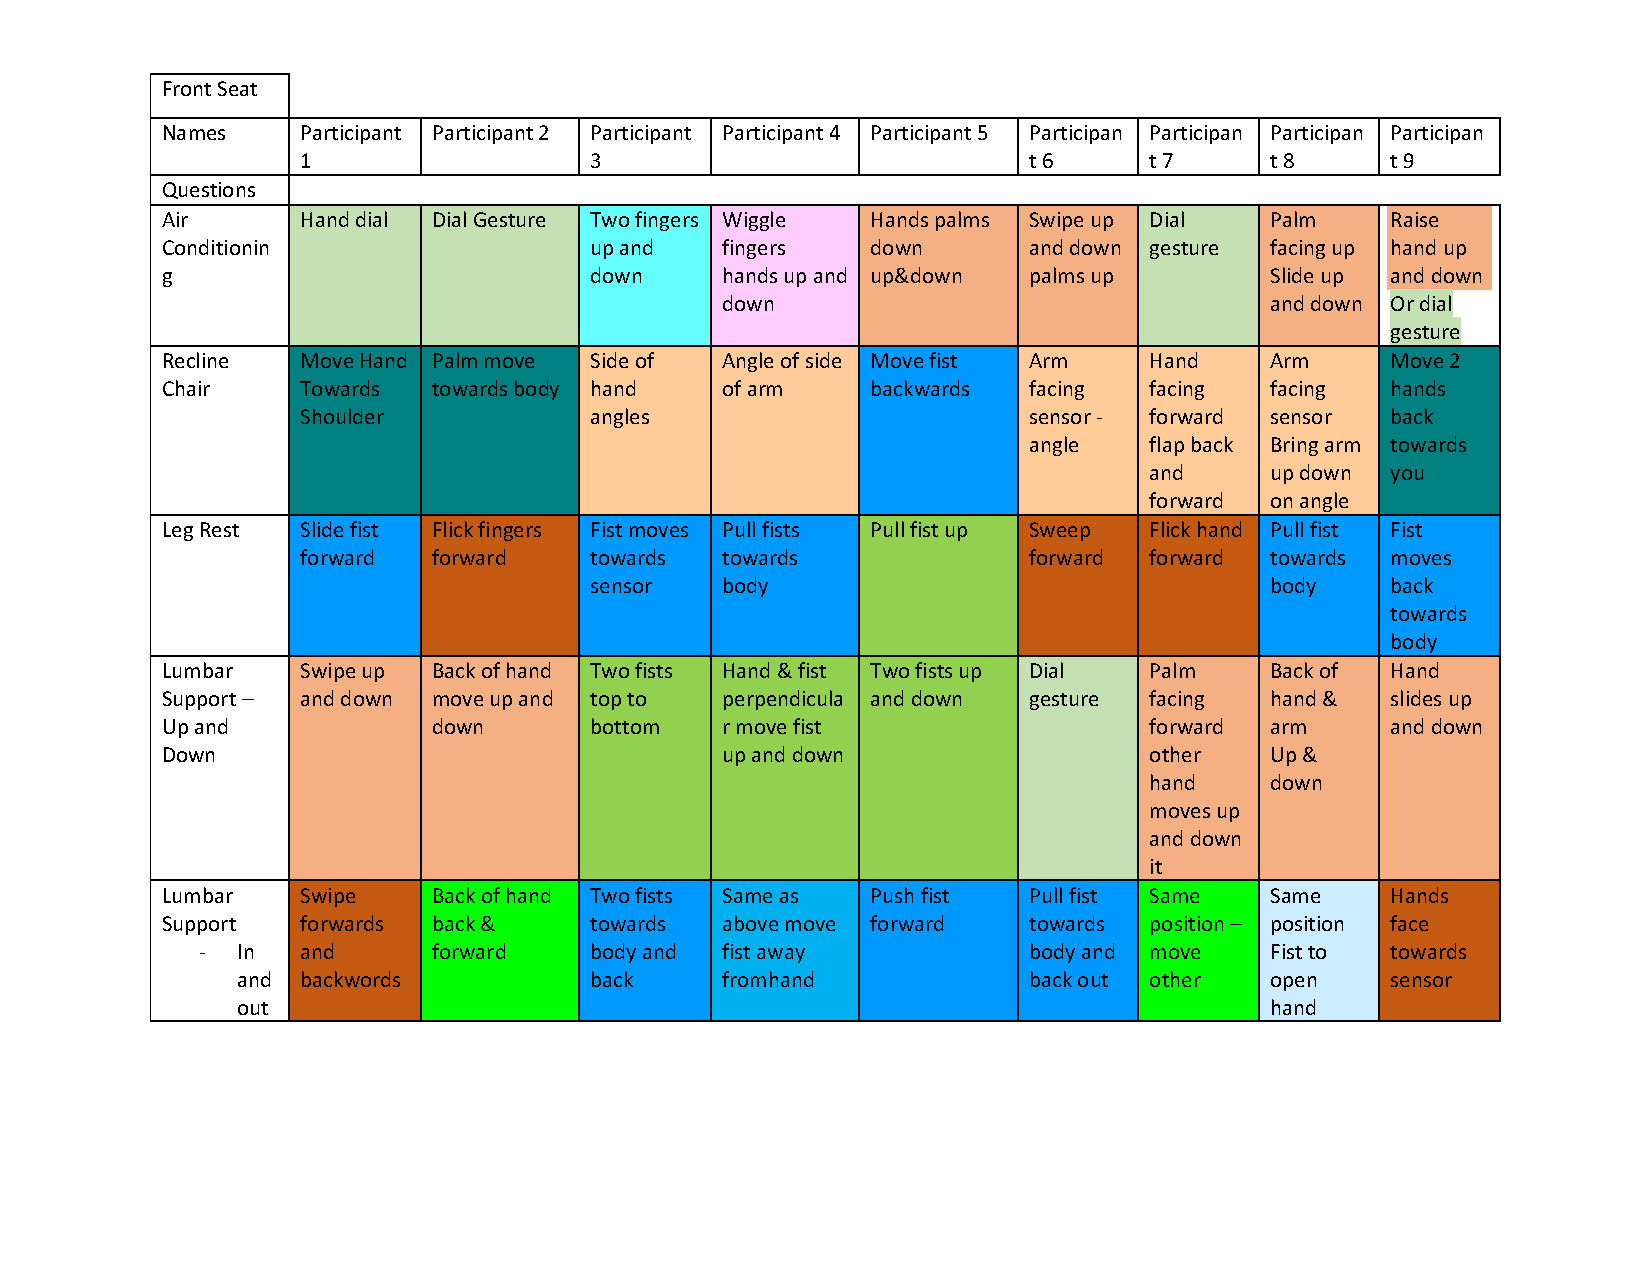
\includepdf[pages=-,pagecommand={},width=\textwidth]{images/PDFs/AnalysisOfGestures.pdf}

\section{Graphs Created from Processed Data of Elicited Gestures}
\label{section:graphsGE}
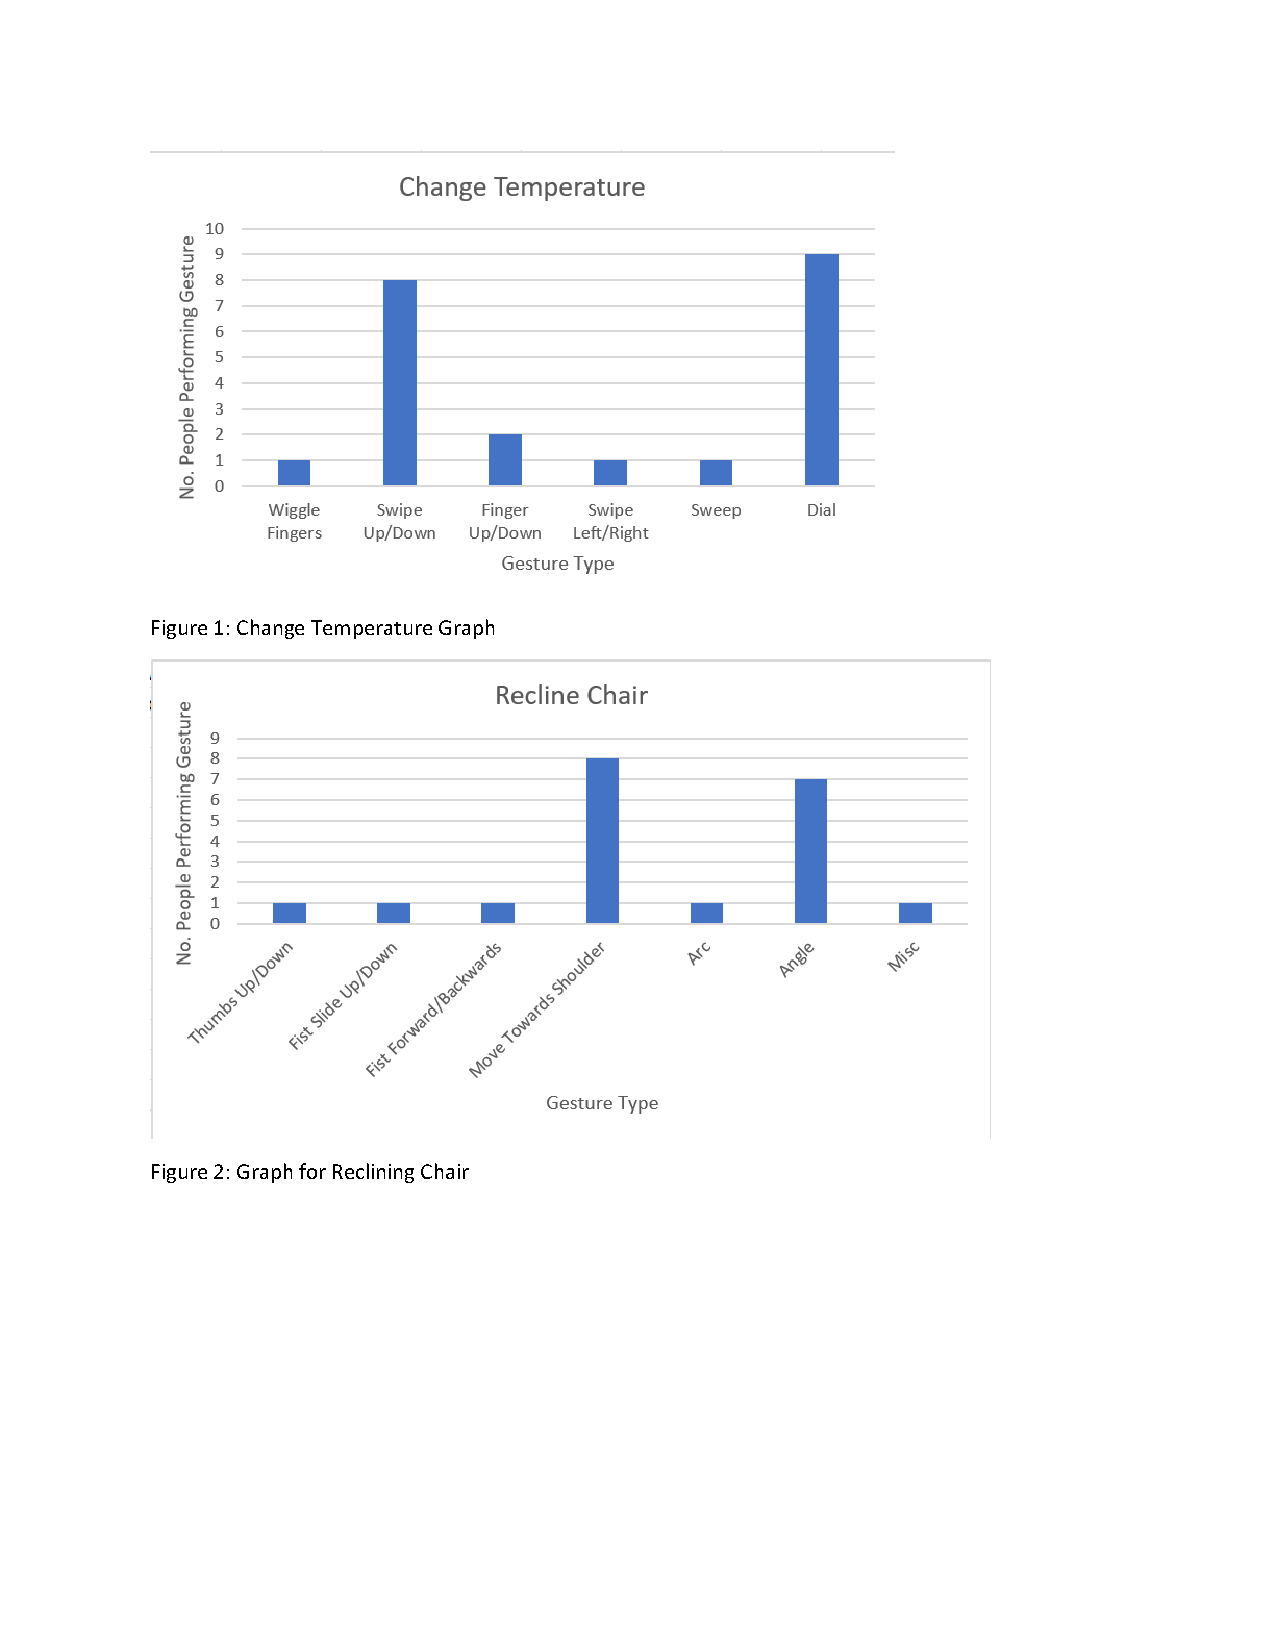
\includepdf[pages=-,pagecommand={},width=\textwidth]{images/PDFs/GraphsofGEResults.pdf}

\chapter{Follow-Up Gesture Elicitation Survey}
\section{Follow-Up Gesture Elicitation Questions}
\label{section:followUpGEQu}
Google Form: \url{https://forms.gle/aPCQwahDUs9B7Aem8}

This survey talked through 21 gestures and asked the same three questions:\\
1. Which gesture do you prefer?\\
2. Rate your chosen gesture from Not Intuitive at all to Very Intuitive (Scale of 1 to 5)\\
3. Is there any gesture you would rather do?\\

\section{Results}
\label{section:followUpGEResults}
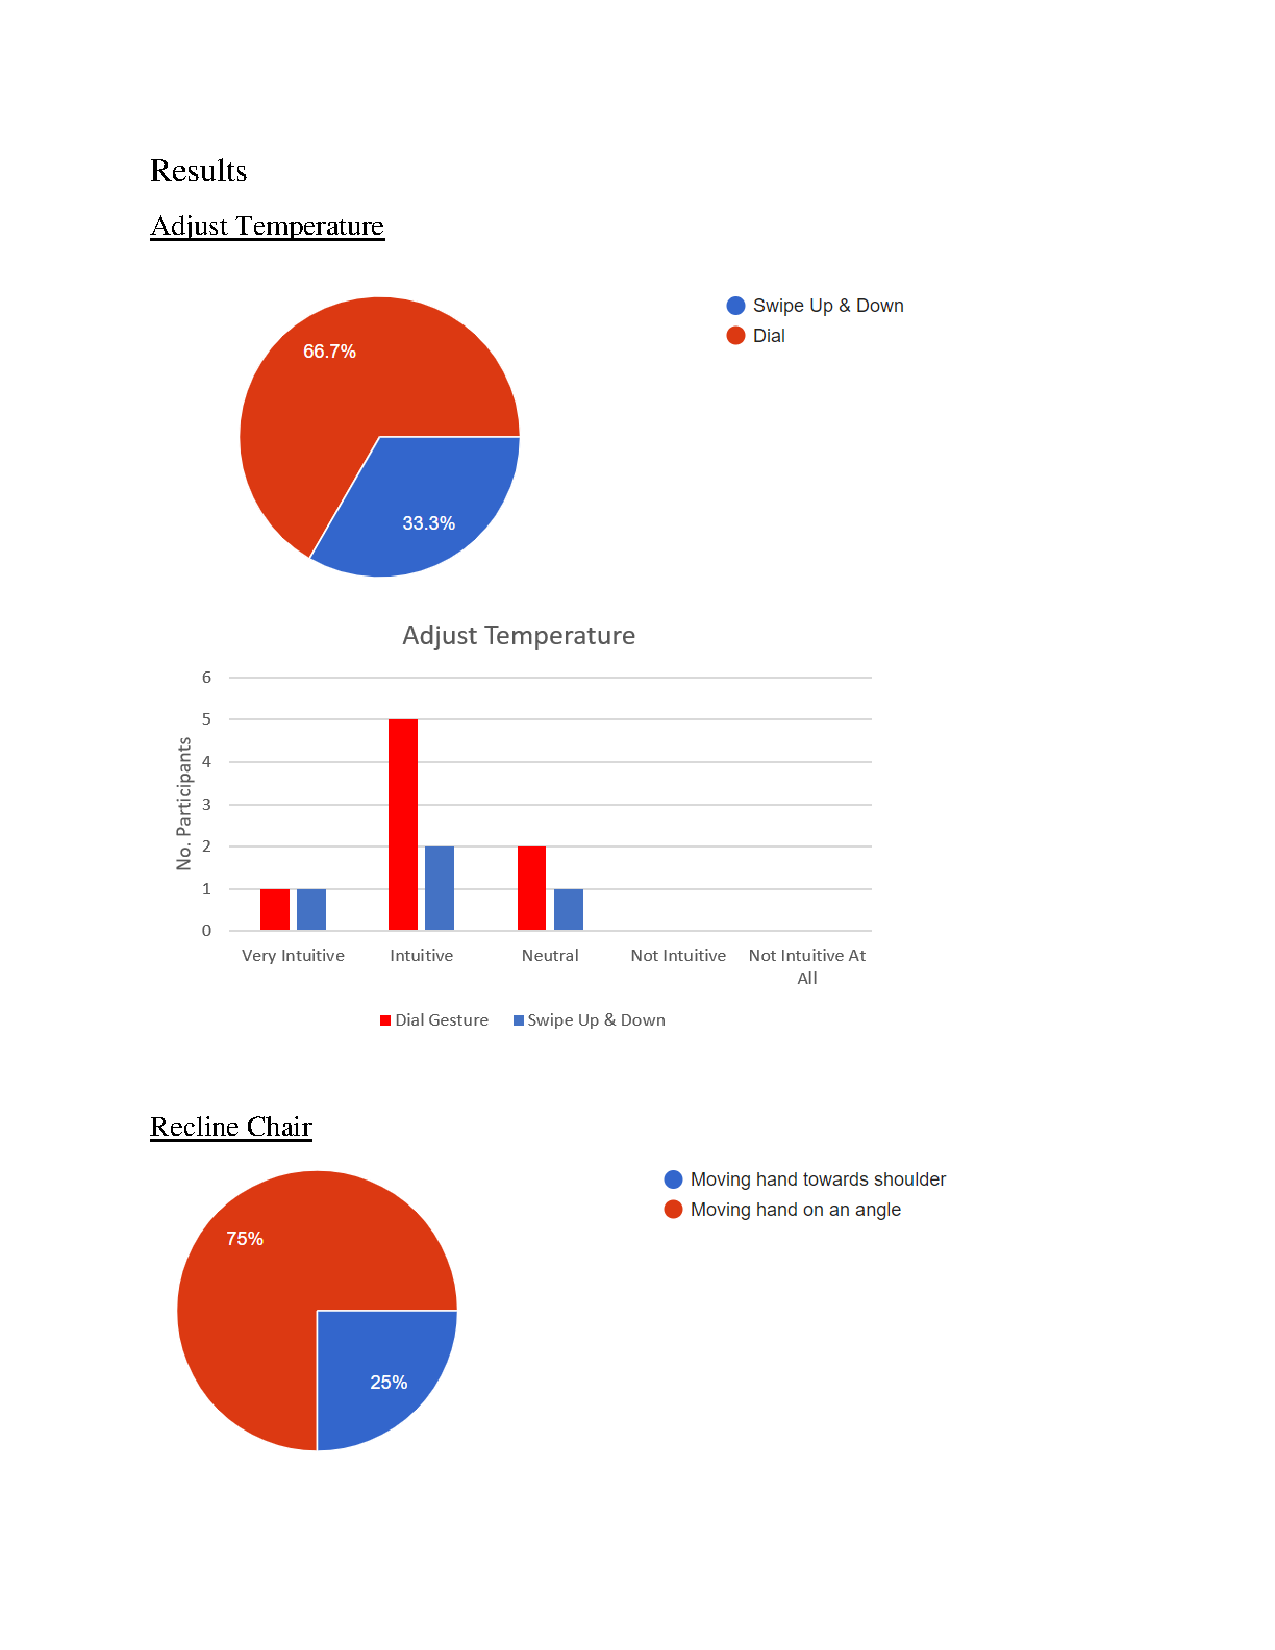
\includepdf[pages=-,pagecommand={},width=\textwidth]{images/PDFs/followUpGEResults.pdf}


\chapter{Design}
\section{Wireframes}
\label{section:wireframes}
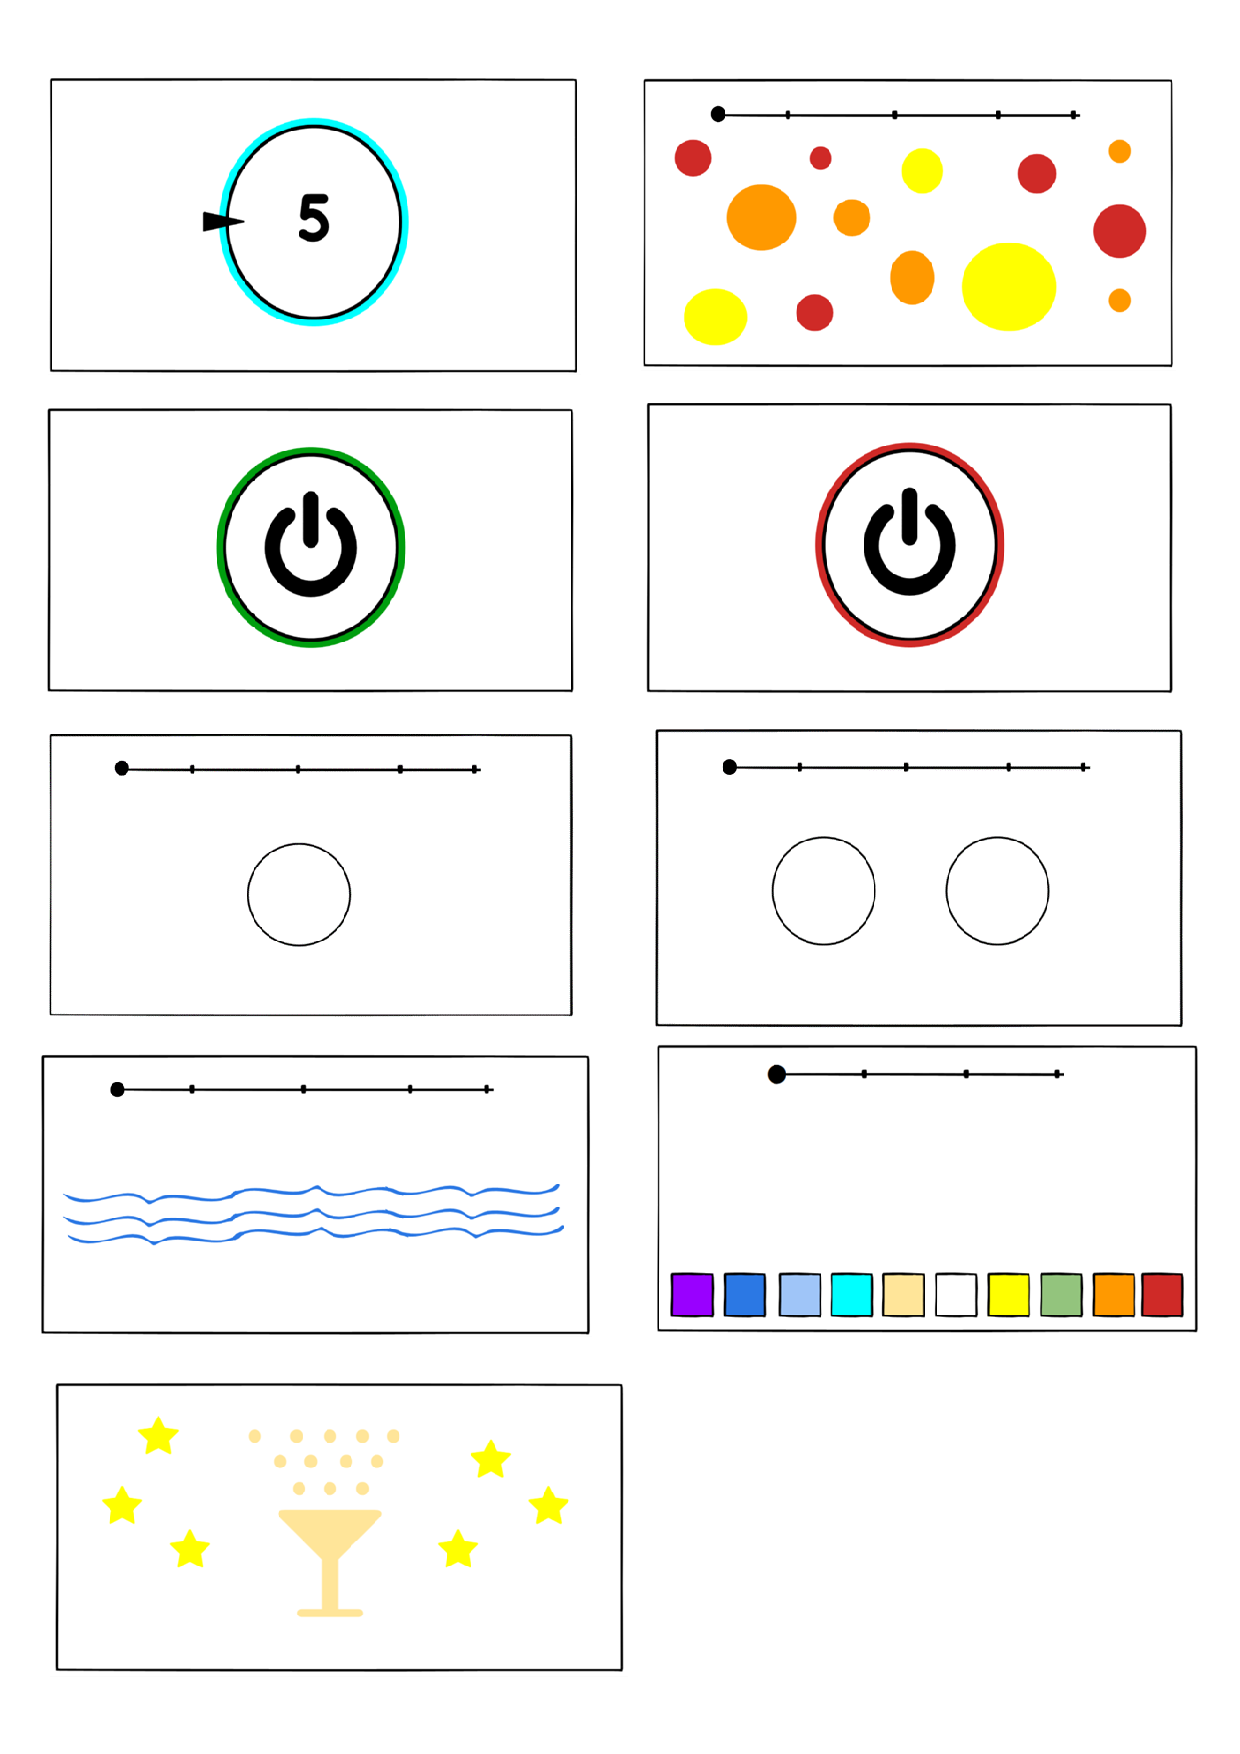
\includepdf[pages=-,pagecommand={},width=\textwidth]{images/PDFs/wireframes.pdf}

\chapter{Experiment}
\section{Signed Ethics Checklist}
\label{section:checklistJan21}
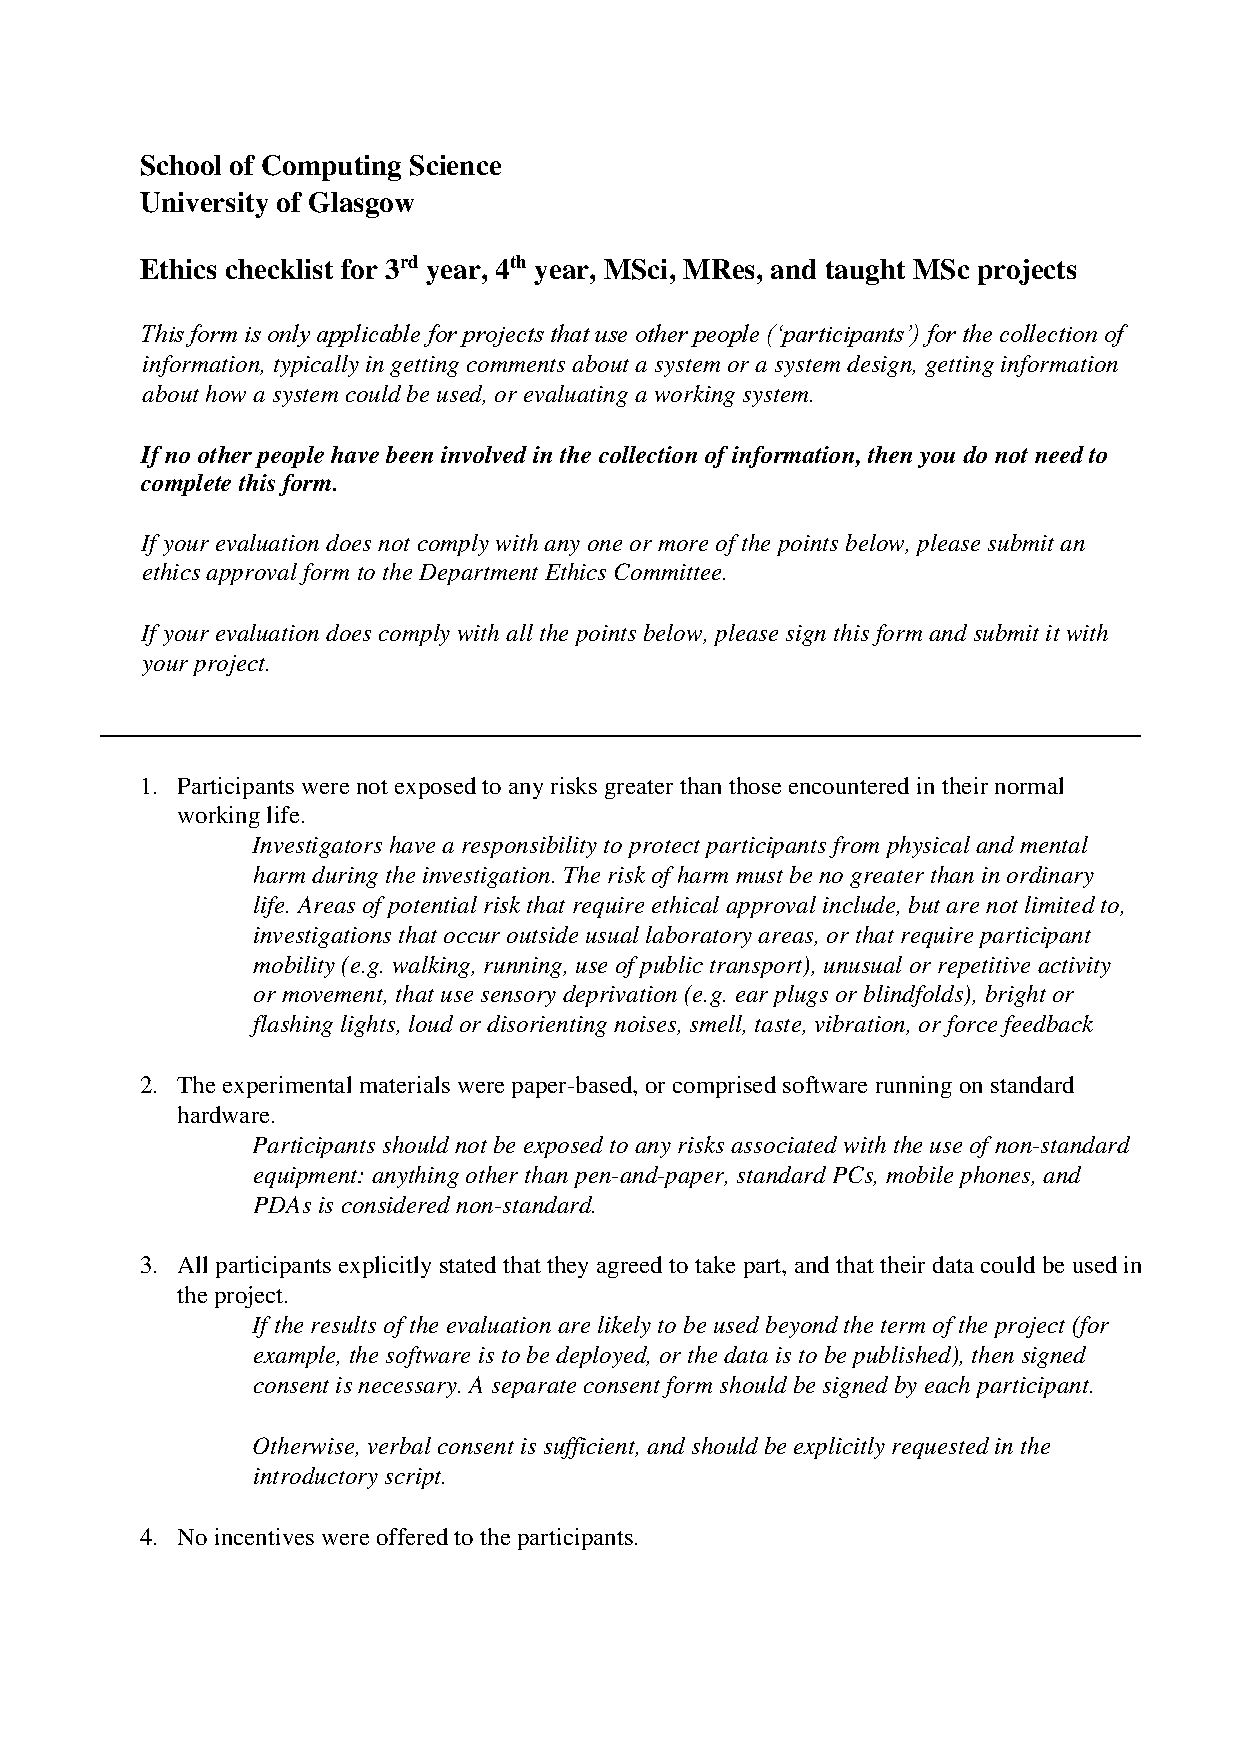
\includepdf[pages=-,pagecommand={},width=\textwidth]{images/PDFs/SignedChecklistExperimentJan2021.pdf}

\section{Participant Consent Form for Experiment}
\label{section:consentExp}
The aim of this experiment is to investigate what gestures are most usable in a car. This survey should take roughly 30 minutes to complete.

Firstly, the format of the survey will be explained, and the participant will be asked to sit in the backseat of the car with a laptop in front of them.

All results will be kept private and no personal information will be stored about the participant. If they choose to drop out, then all data will be discarded.

\begin{tabbing}
If you \=have any further questions about the survey, please contact:\\
\> Catriona Murphy\\

\>School of Computing Science\\

\>2312695m@student.gla.ac.uk\\

\end{tabbing}

I have read this information sheet, and agree to voluntarily take part in this experiment.

\textbf{Name:}\\
\textbf{Email:}\\
\textbf{Date:}\\


\emph{This study adheres to the BPS ethical guidelines, and has been approved by the DCS ethics committee of The University of Glasgow.. Whilst you are free to discuss your participation in this study with the experimenter, if you would like to speak to someone not involved in the study, you may contact the chair of the DCS Ethics Committee: Prof Stephen Brewster}

\section{Introduction Script for Experiment}
\label{section:introScriptExp}

Introduction Script –Experiment
Mid-Air Geture Interaction in Cars

The general aim of this experiment is to learn about what gestures can be used best in the car for backseat passengers. Your participation is required so that I can see what gestures work best in this scenario.

The experiment will require you to sit in the backseat of my car with my laptop sitting in front of you on the centre console. The reason why you must sit in the middle is so that my laptop can be balanced in the middle console. You will also need to wear a seatbelt for a more realistic participation.

You will be asked to perform a series of gestures. Before each scenario, I will demonstrate how to do the gesture. Between each scenario, you will be asked to fill out a survey to measure the workload of each gesture.

At the end of the experiment, you will be asked to fill out a general questionnaire about your opinions on the experiment.

Do you agree to take part in this experiment?

Do you have any questions before we start?
\cleardoublepage 
\section{TLX Information Sheet Provided to Participants During Experiment}
\label{section:TLXInfoSheet}
A few comments on workload estimation

Workload is difficult to define precisely but easy to understand generally. The factors that influence your experiences in the experiment may come from the experiment itself, your feelings about your own performance, how much effort you put in, or the stress and frustration you felt. The workload contributed by these different factors may change as you get more familiar with the experiment. The physical parts of workload are easy to measure but the mental ones are harder.

Since workload is something that is experienced individually by each person, there are no effective measures that can be used to estimate the workload of different activities. One way to find out about workload is to ask people to describe the feelings they experienced. Because workload may be caused by many different factors, we would like you to evaluate several of them individually. This set of 7 scales was developed for you to use in evaluating your experiences in different tasks. Please read the definitions of the scales carefully. If you have a question about any of the scales in the table please ask me about it. It is extremely important that they be clear to you. You may keep the descriptions with you during the experiment.
\begin{figure}[!htb]
    \centering
    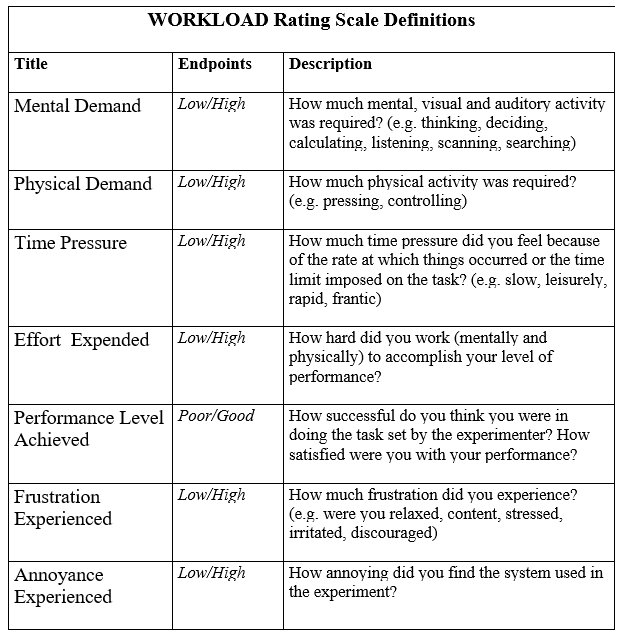
\includegraphics[scale = 0.6]{images/workload.png}
\end{figure}

After each section of the experiment you will be asked you to fill in the 7 scales. You will evaluate the condition by marking each scale at the point which matches your experience. Each line has a description at each end. Please consider your responses carefully. Consider each scale individually. Your ratings will play an important role in the evaluation being conducted, thus your active participation is essential to the success of this experiment, and is greatly appreciated.

\section{Debrief Script for Experiment}
\label{section:debriefExp}
Debrief Script –Experiment

Mid-Air Gesture Interaction in Cars

The main aim of this survey was to find out if the gestures were able to be done in the backseat of the car. However, I was also looking to see if the feedback given was appropriate. If it wasn't then I would have to look into other ways to give feedback.

Do you have any comments or questions about the survey?

If you do have any further questions then you have my contact details. Thank you for your help.

\section{Experiment Survey \& Follow-Up Survey}
\label{section:expSurvey}
Experiment Survey: \url{https://forms.gle/nHpewv98C1uJGptC7}\\
Follow-Up Survey: \url{https://forms.gle/X6hXebP4EFHiPQ5S8}


\section{TLX Results}
\label{section:TLXResults}
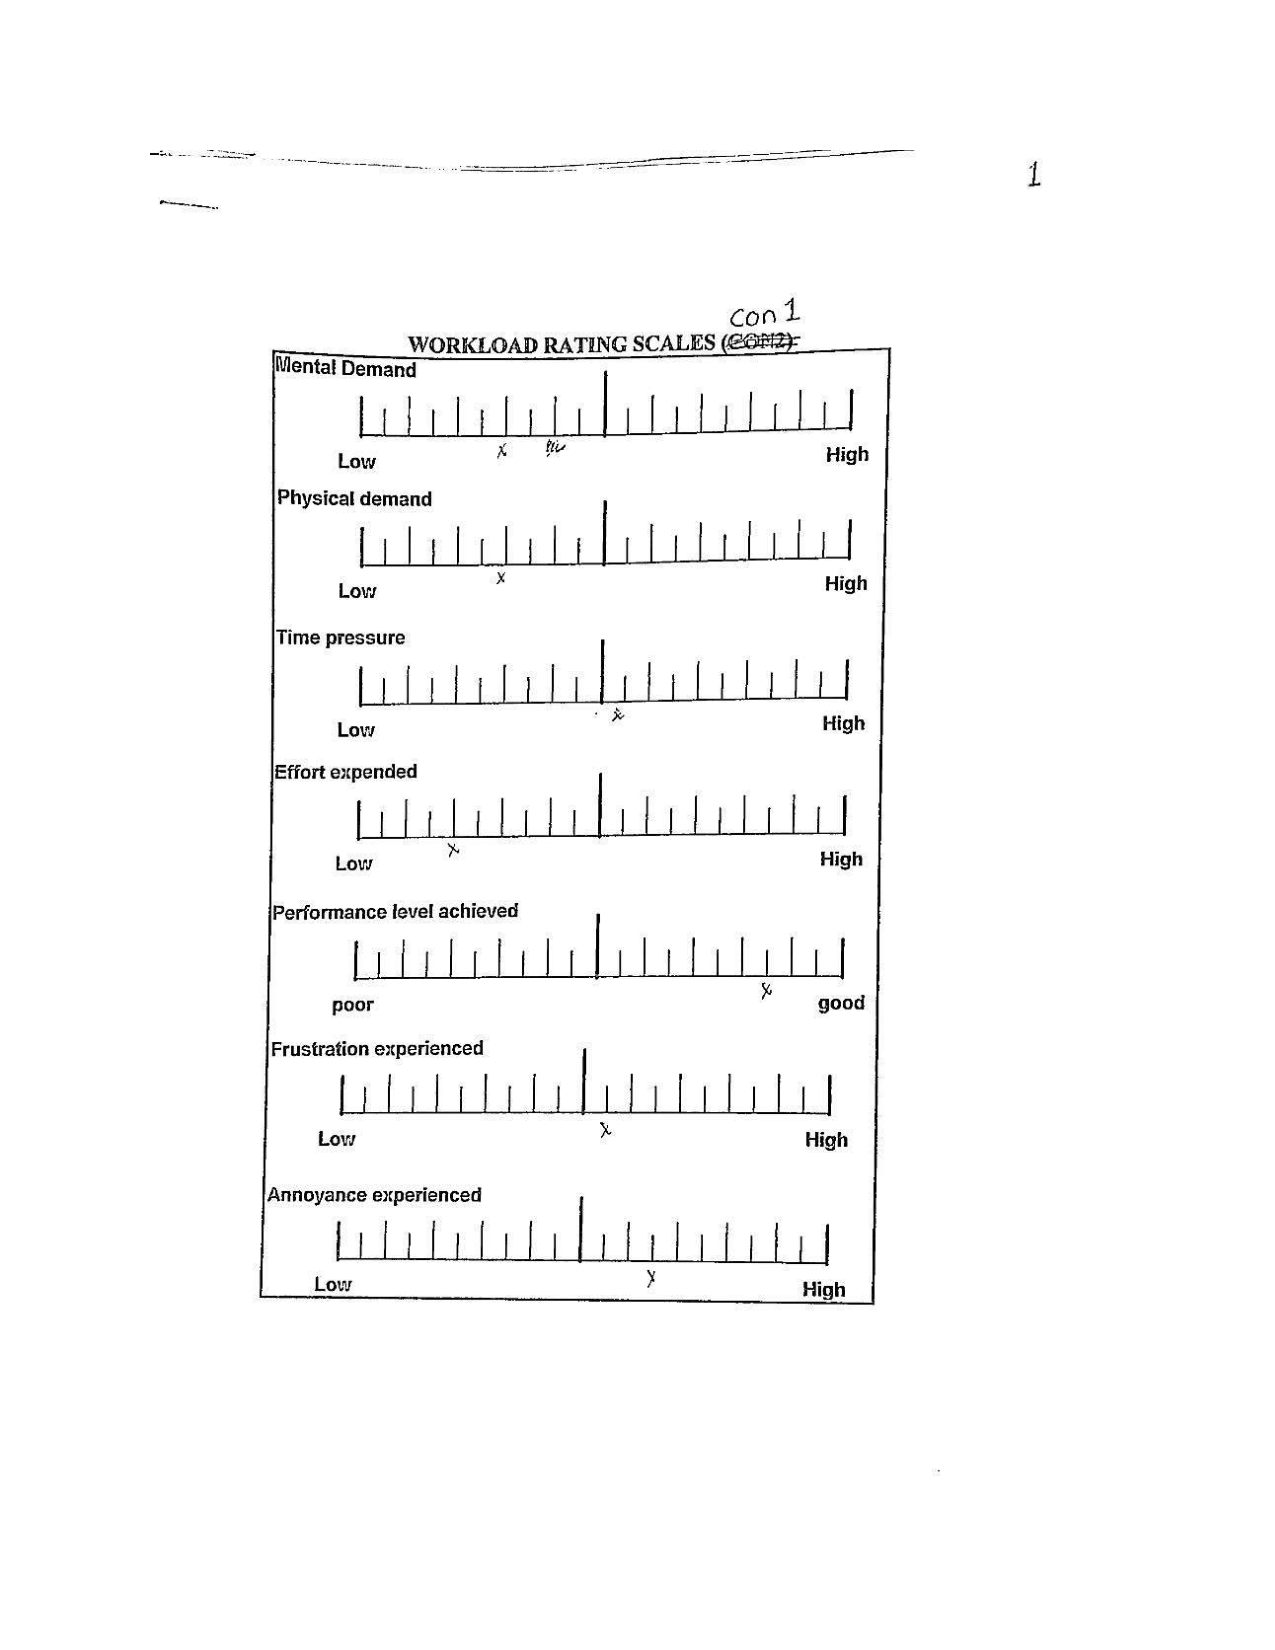
\includepdf[pages=-,pagecommand={},width=\textwidth]{images/PDFs/TLXResults.pdf}


\section{TLX Results Graphs}
\label{section:TLXGraphs}
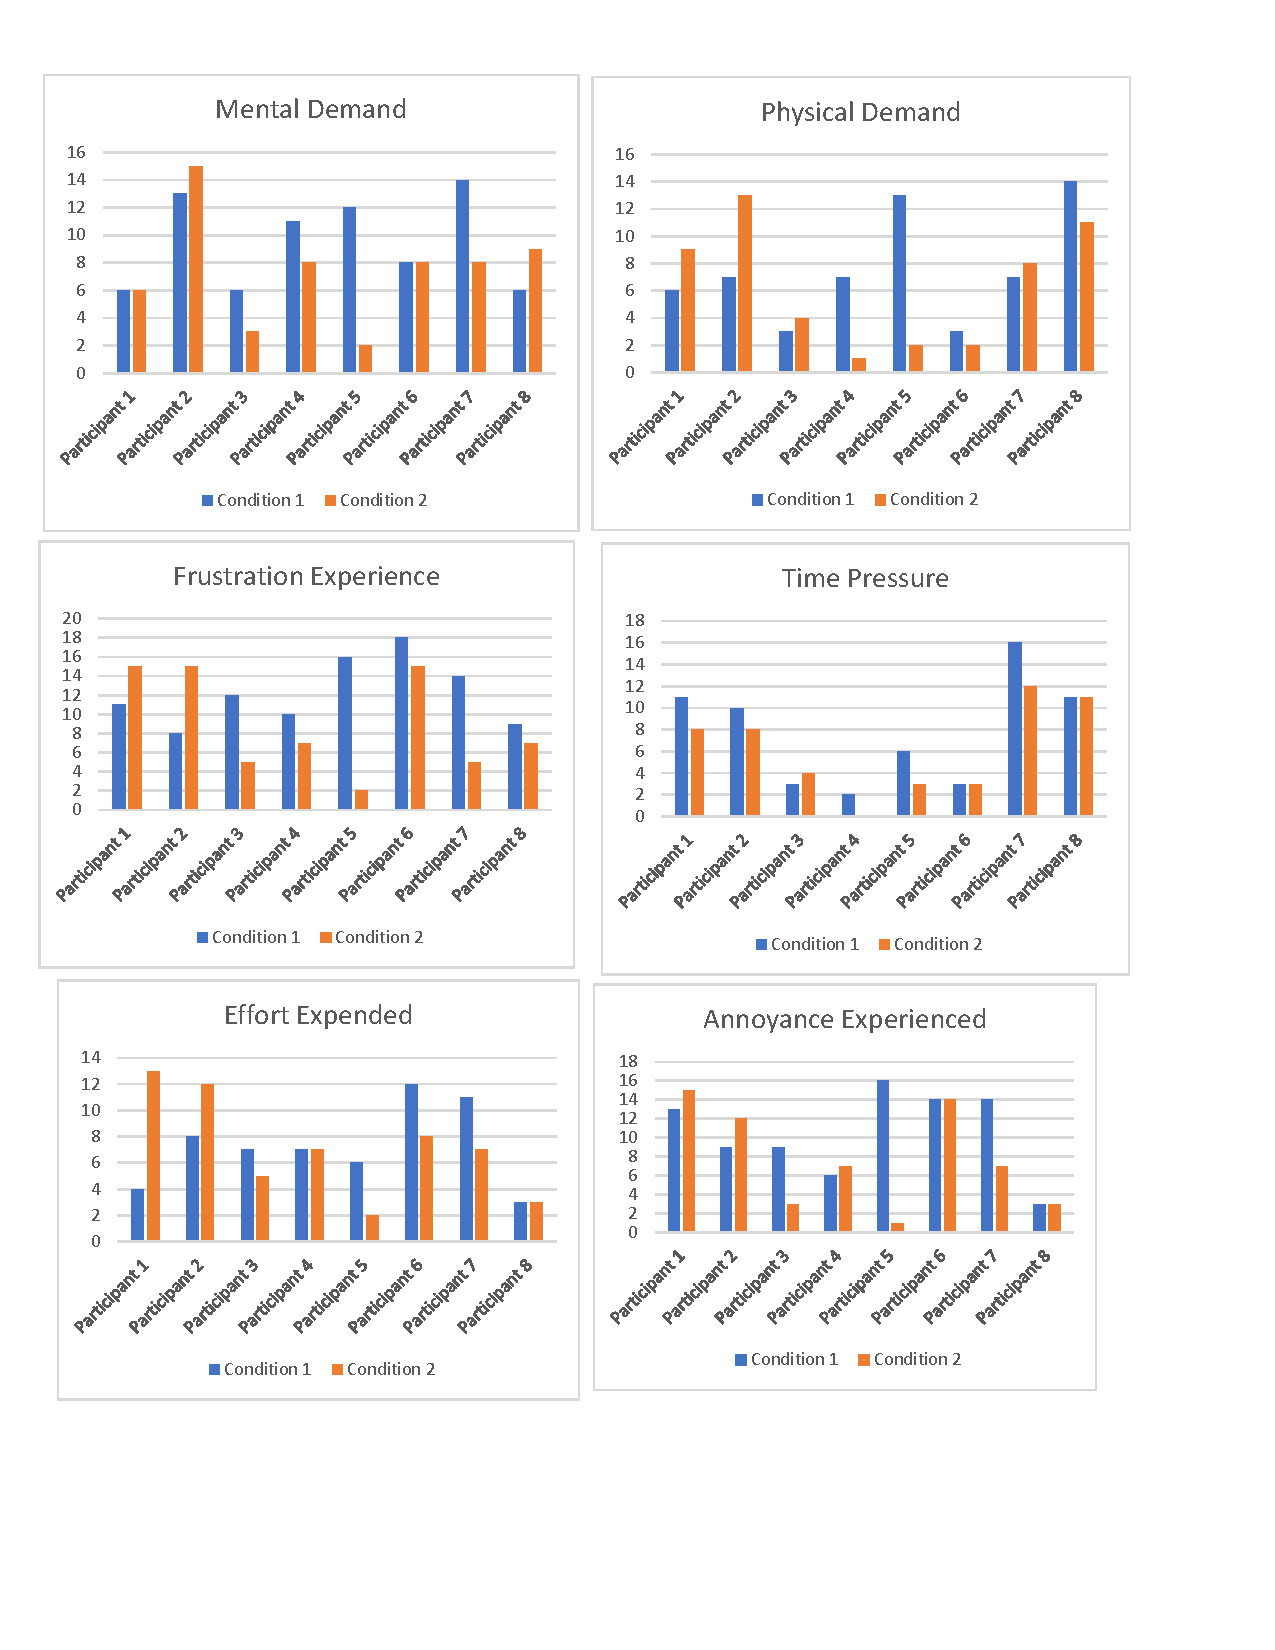
\includepdf[pages=-,pagecommand={},width=\textwidth]{images/PDFs/workload.pdf}

\end{appendices}

%==================================================================================================================================
%   BIBLIOGRAPHY   

% The bibliography style is agsm (Harvard)
% The bibliography always appears last, after the appendices.

\bibliographystyle{agsm}

% Force the bibliography not to be numbered
\renewcommand{\thechapter}{0} 
\bibliography{l4proj}

\end{document}
